\documentclass[Bachelor, Submit, UKenglish, ngerman]{scrbook}
%------------------------------------------------------------------------------
% This file contains a skeleton thesis for
% a Physics or Astronomy Institute in the University of Bonn.

% Specify the thesis type as an option: PhD, Master, Diplom, Bachelor.
% Specify the thesis stage as an option: Draft (default), Submit, Final, PILibrary.

% Specify the language(s) in the class and then use babel.
% If you need more than one language, give the default language last,
% e.g. ngerman, UKenglish for a thesis in British (UK) English where you want
% to be able to set the language to German for some part of it.

%------------------------------------------------------------------------------
% Pass TeX Live version to the package.
% Use command pdflatex --version to find out which version you are running.
% twoside=true is suitable for printing, while twoside=false is probably better for PDF version.
\usepackage[twoside=true, texlive=2017]{ubonn-thesis}

%------------------------------------------------------------------------------
% Adjustments to standard biblatex style.
% Change option to backref=false when your thesis is ready to turn off back-referencing.
% Pass the option showurl=false to shorten your bibliography by not including url fields.
\usepackage[backref=true]{ubonn-biblatex}

%------------------------------------------------------------------------------
% Glossary package
% \usepackage[acronym,toc,nosuper]{glossaries}
% TikZ packages and libraries
% \usepackage{tikz}
% \usepackage{tikz-3dplot}
% \usepackage{pgfplots}
% \usetikzlibrary{positioning,shapes,arrows}
% \usetikzlibrary{decorations.pathmorphing}
% \usetikzlibrary{decorations.markings}
\usepackage{thesis_defs}

%------------------------------------------------------------------------------
% Instead of colouring  links, cites, table of contents etc.
% put them in a coloured box for the screen version.
% This is probably a good idea when you print your thesis.
% \hypersetup{colorlinks=false,
%   linkbordercolor=blue,citebordercolor=magenta,urlbordercolor=darkgreen
% }

%------------------------------------------------------------------------------
% When writing your thesis it is often helpful to have the date and
% time in the output file. Comment this out for the final version.
%\ifoot[\today{} \thistime]{\today{} \thistime}

% In order to check if your labels are referenced try the refcheck package
% \usepackage{refcheck}

%------------------------------------------------------------------------------
% MY PACKAGES
\usepackage{mathrsfs}   % for the functional integral measure D[x]
\usepackage{listings}   % for code listings
\usepackage{dsfont}     % for the unit matrix \mathds{1}
\usepackage{algorithm}  % for the environment for pseudo code
\usepackage{algorithmic}% for the pseudo code itself
\usepackage[stable]{footmisc} % for footnotes in section titles

\lstset{
  basicstyle=\small,
  columns=fullflexible,
  frame=single,
  breaklines=true,
  postbreak=\mbox{\textcolor{red}{$\hookrightarrow$}\space},
  showstringspaces=false,
  numbers=left,
}
\interfootnotelinepenalty=10000 % to prevent page breaks in footnotes

%------------------------------------------------------------------------------
% biblatex is included by ubonn-thesis. Look there for the settings used.
% See the options for settings that can be changed easily.
% For further changes copy the \RequirePackage[...]{biblatex} here
% and include ubonn-thesis with the option biblatex=false.

% Specify the bibliography files here and not at the end!
% Use standard_refs-bibtex if you use bibtex or bibtex8
% and standard_refs-biber  if you use biber
\addbibresource{bib/thesis_refs.bib}
\addbibresource{bib/standard_refs-biber.bib}

%------------------------------------------------------------------------------
% The following definitions are used to produce the title pages
% needed at various stages
\newcommand{\thesistitle}{Untersuchung von Quantensystemen mit Hilfe von gitterfeldtheoretischen Methoden}
\newcommand*{\thesisauthor}{Heinrich v. Campe}
\newcommand*{\thesistown}{Crivitz}
\renewcommand*{\InstituteName}{\HISKP}
\renewcommand*{\inInstitute}{\inHISKP}
\renewcommand*{\InstituteAddress}{\HISKPaddress}
% Adjust \thesisreferee...text depending on male/female referee
\newcommand*{\thesisrefereeonetext}{1.\ Gutachter}
\newcommand*{\thesisrefereeone}{Prof.\ Dr.\ Carsten Urbach}
\newcommand*{\thesisrefereetwotext}{2.\ Gutachter}
\newcommand*{\thesisrefereetwo}{Prof.\ Dr.\ Thomas Luu}
% Date when thesis was submitted (Master/Diplom)
% Year or Month, Year when thesis was submitted (PhD)
\newcommand*{\thesissubmit}{06.09.2021}
% \newcommand*{\thesissubmit}{Month 2021}
% Date of thesis examination (PhD)
\newcommand*{\thesispromotion}{XX.YY.2021}
% Month and year of the final printed version of the thesis
\newcommand*{\thesismonth}{September}
\newcommand*{\thesisyear}{2021}
\newcommand*{\thesisnumber}{BONN-IR-2021-09}
% Dedication
% \newcommand*{\thesisdedication}{}

%------------------------------------------------------------------------------
% The abstract is only needed for the printed version and should be in
% English regardless of the language of the thesis
\newcommand{\thesisabstract}{%
  \begin{otherlanguage}{UKenglish}
    This is your thesis abstract. It may be in a language that is
    different from the rest of your thesis.
  \end{otherlanguage}
}

%------------------------------------------------------------------------------
% MY COMMANDS
%\newcommand{\su2}{SU(2)} % does not work yet.

%------------------------------------------------------------------------------
% \includeonly can be used to select which chapters you want to process
% A simple \include command just inserts a \clearpage before and after the file
% Note that \includeonly can be quite picky! Do not forget to put a
% comma after the filename, otherwise it will simply be ignored!
% \includeonly{%
%   thesis_intro,
%   thesis_appendix,
%   thesis_acknowledge
% }

%------------------------------------------------------------------------------
% Give a list of directories where figures can be found. Do not leave
% any spaces in the list and end the directory name with a /
\graphicspath{%
  {figs/}%
  {figs/cover/}%
}

%------------------------------------------------------------------------------
% Make a glossary and a list of acronyms
% \makeglossaries

% Glossary entries
% \input{thesis_glossary}

% Draft version - add the word DRAFT on the cover pages
\ifthenelse{\equal{\ThesisVersion}{Draft}}{%
  \usepackage{background}
  \backgroundsetup{contents=DRAFT, color=blue!30}
}

%------------------------------------------------------------------------------
\begin{document}

% Make cover and title pages
\makethesistitle

\pagestyle{scrplain}

%------------------------------------------------------------------------------
% You can add your acknowledgements here - don't forget to also add
% them to \includeonly above
% %------------------------------------------------------------------------------
\chapter*{Acknowledgements}
\label{sec:ack}
%------------------------------------------------------------------------------

I would like to thank ...

You should probably use \texttt{\textbackslash chapter*} for
acknowledgements at the beginning of a thesis and
\texttt{\textbackslash chapter} for the end.

%%% Local Variables: 
%%% mode: latex
%%% TeX-master: "../mythesis"
%%% End: 


\tableofcontents

\mainmatter
\pagestyle{scrheadings}

% Turn off DRAFT for the following pages
\ifthenelse{\equal{\ThesisVersion}{Draft}}{%
  \backgroundsetup{contents={}}
}{}

%------------------------------------------------------------------------------
% Add your chapters here - don't forget to also add them to \includeonly above
% !TEX root = mythesis.tex

%==============================================================================
\chapter{Einleitung}
\label{sec:einleitung}
%==============================================================================

Die theoretische Teilchenphysik erfuhr eine Reihe von Durchbrüchen, nachdem
Gell-Mann und Zweig 1964 das Konzept von Quarks eingeführt hatten. So benannten
sie die \enquote{Bausteine} des in den vorherigen Jahren immer größer gewordenen
Teilchenzoos und erklärten insbes. die von Gell-Mann und Ne'eman zuerst beschriebenen
SU(3)-Multiplets von Baryonen~\cite{historyOfQCD}. 1971 führten Gell-Mann und Fritzsch
die Farbladung der Quarks als weitere Quantenzahl ein, um Zustände aus drei
gleichen Quarks mit dem Pauli-Prinzip in Einklang zu bringen. Im darauffolgenden
Jahr betrachteten sie dann die Farb-Gruppe SU(3) als Eichgruppe und legten so
die Grundsteine einer neue Theorie, der Quantenchromodynamik~\cite{historyOfQCD}.
Eine wichtige Eigenschaft dieser neuen Theorie ist das sog. \emph{Confinement}:
Quarks können nie ungebunden auftreten. Rein physikalisch lässt
sich diese Eigenschaft darauf zurückführen, dass Gluonen (die Mediatoren der 
beschriebenen, sog. starken Wechselwirkung) selbst Farbladungen tragen, also anders
als z.\,B. Photonen auch untereinander interagieren können~\cite{latticeQCDhistory}.

Leider hat die Quantenchromodynamik einen beträchtlichen Nachteil gegenüber
der Quantenelektrodynamik: Bei niedrigen Energien lässt sie sich nicht perturbativ
betrachten. Hierdurch sind analytische Betrachtungen in diesem Bereich sehr schwierig,
weswegen andere Methoden vonnöten sind. Eine solche Alternative bietet eine
gitterfeldtheoretische Formulierung, welche erstmals 1974 von Wilson vorgelegt
wurde~\cite{latticeQCDhistory}. Dabei präsentierte er gleichzeitig eine erste
Motivation für Confinement, welche fünf Jahre später numerisch bestätigt werden konnte.

In dieser Arbeit soll diese numerische Betrachtung nachvollzogen
werden: Der Einfachheit halber wird hier nur die SU(2)-Eichsymmetrie betrachtet:
Die Simulation des dazugehörigen Eichfelds bietet die Möglichkeit, den Wert des
statischen Potentials eines Quark\footnote{Am treffendsten wäre wohl die Bezeichnung
als \enquote{Pseudoquark}, da es sich nicht um die SU(3)-Eichsymmetrie
handelt.}-Antiquark-Paars für
verschiedene Abstände zu berechnen. Confinement sollte dann dadurch zu erkennen
sein, dass das Potential (neben einem Coulomb-artigen Verhalten für kleine Abstände)
für große Abstände \emph{linear} ansteigt. Entsprechend bleibt die Kraft zwischen
Quark und Antiquark konstant, wodurch man das Paar nicht voneinander isolieren kann.

Folgender Aufbau wurde für die folgenden Abschnitte gewählt: In Kapitel
\ref{sec:theorie} wird mit dem Metropolisalgorithmus erst die allgemeine
numerische Methode
vorgestellt, welche die numerische Approximation von Feynmans Pfadintegralen
ermöglicht. Darauf folgt dann die theoretische Anwendung auf die SU(2)-Eichsymmetrie
-- von einer allgemeinen Formulierung der Wirkung zur konkreten Observable für die 
Bestimmung des statischen Potentials. Kapitel \ref{sec:implementation}
enthält dann die Details der konkreten Implementation und den Ablauf der 
Simulation und in Kapitel \ref{sec:auswertung} werden die gewonnenen
Daten ausgewertet und die Ergebnisse präsentiert.


% !TEX root = mythesis.tex

%==============================================================================
\chapter{Theorie}
\label{sec:theorie}
%==============================================================================


\section{Vom Pfadintegral zum Metropolis-Algorithmus}
\subsection{Feynman}
Ausgangspunkt für die verwendete Methode ist der im Rahmen des Feynman'schen
Pfadintegralformalismus eingeführte Propagator \cite{freedmanCreutz}
\begin{equation} \label{eq:propagator}
    \bra{f} e^{-H t} \ket{i} = \int \mathscr{D}[x] e^{-S[x]},
\end{equation}
welcher den Übergang eines physikalischen Systems, charakterisiert durch den
Hamiltonian $H$ resp. der Wirkung $S$,  beschreibt. $x(t)$ sei hier eine
Funktion, welche die Trajektorie des Systems vom Anfangszustand $\ket{i}$ in
den Endzustand $\ket{f}$ charakterisiert, $\int \mathscr{D}[x]$ bezeichne die
Integration über alle Trajektorien. Die berechnete Amplitude setzt sich also
aus allen möglichen Pfaden zusammen, die das System wählen kann, jeder dieser
Pfade $x(t)$ wird mit dem exponentiellen Faktor $e^{-S[x]}$ gewichtet.

In der hier notierten Form wurde
$\hbar = 1$ angenommen sowie die Wick-Rotation zu imaginärer Zeit
\[
    t \mapsto it
\]
verwendet. Letzteres hat den Vorteil, dass anstelle von (womöglich stark
oszillierenden) Phasen nur exponentielle Faktoren betrachtet werden müssen, was
insbes. die Berechnungen mit numerischen Methoden vereinfacht. \cite{freedmanCreutz}

Der Erwartungswert einer Observablen $O$ ist im Rahmen dieses Formalismus'
wie folgt definiert \cite{freedmanCreutz}:
\[
    \langle O \rangle = \frac{1}{Z} \int \mathscr{D}[x] O[x] e^{-S[x]}.
\]
Hierbei ist
\[
    Z = \int \mathscr{D}[x] e^{-S[x]}.
\]
Solche Observablen $O$ sollen schlussendlich gemessen werden. Es fällt auf, dass
diese Definition der eines Erwartungswertes von $O[x]$ bzgl. der Verteilung
\cite{freedmanCreutz}
\begin{equation} \label{eq:feynmanDensity}
    P^\text{Feyn} \mathscr{D}[x] =  \frac{1}{Z} e^{-S[x]} \mathscr{D}[x]
\end{equation}
entspricht. Um diesen Erwartungswert anzunähern, sollen Trajektorien
$\{x^\alpha\}$ aus dieser Verteilung gezogen werden. Dann kann
$\langle O \rangle$ über das arithmetische Mittel zu
\[
    \overline{O} = \frac{1}{N} \sum_{\alpha=1}^N O[x^\alpha]
\]
abgeschätzt werden. $\langle O \rangle$ kann durch Erhöhung der Stichprobengröße
$N$ beliebig gut durch $\overline{O}$ approximiert werden.

Dieser Ansatz vereinfacht die gestellte Aufgabe enorm: Anstelle der Berechnung
eines unendlichdimensionalen Integrals zum Finden von $\langle O \rangle$
muss lediglich eine Menge von Trajektorien $\{x^\alpha\}$ generiert werden, die
der Verteilung folgt. Das soll das nächste Etappenziel sein.

\subsection{Markov}
Eine Möglichkeit, Elemente aus einer bestimmten Verteilung zu ziehen, 
bietet ein iterativer stochastischer Prozess, der als Markov-Kette bezeichnet
wird. Die Betrachtung hier ist an die von Freedman und Creutz \cite{freedmanCreutz}
angelehnt.

Sei zunächst $x$ eine kontinuierliche Größe, welche den Zustand eines
stochastischen Systems beschreibt. $W(x,x')$ ist dann eine Funktion,
welche die Übergangswahrscheinlichkeit des Systems vom Zustand $x$ in den Zustand
$x'$ wiedergibt. Da es sich um eine Wahrscheinlichkeitsdichte handelt, muss
\begin{equation} \label{eq:transitionProb}
    W(x,x') \geq 0\, \forall x, x'
    \text{ und }
    \int \dd{x'} W(x,x') = 1\, \forall x
\end{equation}
gelten. Die zweite Gleichung entspricht der Aussage, dass das System immer in
irgendeinen Zustand übergehen muss, um Wahrscheinlichkeitserhaltung zu
gewährleisten.

Ein $n$-schrittiger Übergangsprozess von $x$ nach $x'$ über $n-1$
Zwischenzustände lässt sich dann durch folgendes Integral beschreiben:
\begin{align*}
    W^{(n)}(x,x') &= \int \dd{x_1} \dd{x_2} \dots \dd{x_{n-1}}
        W(x,x_1) W(x_1, x_2) \dots W(x_{n-2}, x_{n-1}) W(x_{n-1},x')\\
    &= \int \dd{\tilde{x}} W^{(n-1)}(x, \tilde{x}) W(\tilde{x}, x').
\end{align*}
Nun lässt sich zeigen, dass für große $n$ ein Gleichgewichtszustand erreicht
wird, der nicht mehr vom Anfangszustand abhängt \cite{freedmanCreutz}:
\[
\lim_{n \rightarrow \infty} W^{(n)}(x,x') = P(x').
\]
Den Beweis hierfür liefern Freedman und Creutz \cite{freedmanCreutz}.
$P(x')$ ist dann ein \enquote{Eigenvektor} von $W(x,x')$, wie sich durch iteratives
Einsetzen der Definition leicht nachvollziehen lässt:
\[
P(x') 
= \lim_{n+1 \rightarrow \infty} W^{(n+1)}(x,x')
= \lim_{n \rightarrow \infty} \int \dd{x_n} W^{(n)}(x, x_n) W(x_n,x')
= \int \dd{\tilde{x}} P(\tilde{x}) W(\tilde{x},x').
\]
Daher rührt auch die Bezeichnung als Gleichgewichtszustand: Haben wir ein
Verfahren, dass $x'$ aus $x$ erzeugt, wobei die für $W(x,x')$ geforderten Eigenschaften
erfüllt werden, und ist die Konfiguration $x$
erst einmal in einem Zustand, der durch $P(x)$ beschrieben wird, gilt dies auch
für alle durch weitere Iterationen erzeugten Zustände $x'$. Indes muss natürlich
nicht $x' = x$ gelten, lediglich $P(x') = P(x)$ ist garantiert.

Da $W(x,x')$ eine
Wahrscheinlichkeitsdichte ist, gilt dies auch für $P(x')$. Die Idee ist
nun, $W(x,x')$ so zu gestalten, dass wir nach vielen Iterationen von $W(x,x')$
die gewünschte Verteilung $P^\text{Feyn}$ \eqref{eq:feynmanDensity} erhalten.
Hierfür wollen wir zunächst die Eigenschaft der sog. \emph{Detailed Balance}
einführen. Sie besagt \cite{freedmanCreutz}:
\begin{equation} \label{eq:detailedBalance}
\frac{W(x,x')}{W(x',x)} = \frac{P(x')}{P(x)}.
\end{equation}
Hierdurch wird die o.\,g. Eigenwertgleichung impliziert:
\[
\int \dd{x} P(x) W(x,x') = \int \dd{x} P(x) \frac{P(x')}{P(x)} W(x',x)
= P(x') \underbrace{\int \dd{x} W(x',x)}_{= 1 \, \eqref{eq:transitionProb}}.
\]
Setzen wir in die Detailed Balance Bedingung \eqref{eq:detailedBalance} die
Definition der gewünschten Wahrscheinlichkeitsdichte \eqref{eq:feynmanDensity}
ein, so finden wir
\[
\frac{W(x,x')}{W(x',x)} = \frac{e^{-S[x']}}{e^{-S[x]}}
\eqqcolon e^{-\Delta S[x',x]}
\]
als Anforderung an das Verfahren zur Erzeugung von $x'$ aus $x$.

\subsection{Metropolis} \label{sec:metropolis}
So ein Verfahren ist der Metropolis-Algorithmus. Seine grundsätzliche Funktionsweise
ist in Algorithm \ref{alg:metropolis} nachzulesen. Um sie zu verstehen,
ist es wichtig zu wissen, dass in der numerischen Praxis eine Trajektorie $x$
üblicherweise in irgendeiner Form als ein Array mit Elementen $x_i \in x$ gespeichert
wird.

\begin{algorithm}
    \caption{Metropolissweep} \label{alg:metropolis}
\begin{algorithmic}[0]
    \REQUIRE $x$
    \FOR{$x_i \in x$}
        \STATE generate random $x'_i$
        \STATE compute
        $\Delta S[x'_i, x_i, x] = S[\{\cdots, x_{i-1}, x'_i, x_{i+1}, \cdots\}]\
        - S[\{\cdots, x_{i-1}, x_i, x_{i+1}, \cdots\}]$
        \IF{$\Delta S[x'_i, x_i, x] < 0$}
            \STATE set $x_i = x'_i$
        \ELSE
            \STATE draw random $r \in U(0,1)$
            \IF{$r < e^{-\Delta S[x'_i, x_i, x]}$}
                \STATE set $x_i = x'_i$
            \ENDIF
        \ENDIF
    \ENDFOR
\end{algorithmic}
\end{algorithm}

Alle Elemente von $x_i \in x$ werden also nacheinander zunächst zufällig
verändert, dann wird jeweils berechnet, wie sich dadurch die Wirkung verändert.
Wird sie kleiner, setzt man $x_i$ auf den neuen Wert. Für den Fall
$\Delta S > 0$ kann $x_i$ trotzdem aktualisiert werden, dann allerdings mit
der Wahrscheinlichkeit $P = e^{-\Delta S}$. (Dies wird in der Praxis durch die
zufällige Ziehung von $r$ aus $(0,1)$ und den Vergleich mit $P$ bewerkstelligt.)
Zusammen gilt also für einen einzelnen Schritt:
\[
W(x,x') =
\begin{cases}
    1 & \text{wenn } \Delta S < 0, \\
    e^{-\Delta S} & \text{sonst}.
\end{cases}
\]
Hiermit wird auch klar, dass der Algorithmus die Detailed Balance-Bedingung
\eqref{eq:detailedBalance} erfüllt: Sei oBdA $S[x'] < S[x]$. Dann ist
\[
W(x,x') = 1, \; W(x',x) = e^{-\left( S[x] - S[x'] \right)}
\rightarrow \frac{W(x,x')}{W(x',x)} = \frac{e^{-S[x']}}{e^{-S[x]}}.
\]
In der Praxis ist der Algorithmus noch in dreierlei Hinsicht verändert: Der
wichtigste Aspekt ist der, dass die \emph{Veränderung} der Wirkung $\Delta S$ durch
die Modifikation eines einzelnen Gitterpunkts $x_i$ oft nur von $x_i, x'_i$ und
den direkten \enquote{Nachbarn} (je nach Topologie des Problems) von $x_i$
abhängt. Dies vereinfacht die auszuführende Rechnung je Gitterpunkt enorm.
Im Gegensatz zum notierten Algorithmus werden die neuen Vorschläge $x'_i$
außerdem \enquote{nah} an den ursprünglichen Positionen $x_i$ gewählt (die Metrik hängt
vom betrachteten Problem ab). Dadurch wird zwar die potentielle Veränderung der
Trajektorie durch eine Iteration kleiner, allerdings erhöht sich so die
Wahrscheinlichkeit, dass der neue Vorschlag $x_i$ vom Algorithmus
\enquote{angenommen} wird. Schließlich werden für jedes $x_i$ mehrere
Iterationen des Algorithmus ausgeführt, bevor zum nächsten Gitterpunkt übergegangen
wird. Hierdurch wird $x_i$ zunächst mit seinen \enquote{Nachbarn} optimal
eingestellt, was auch die allgemeine Konvergenz zum Equilibrium beschleunigt.

\section{Intermezzo: Der harmonische Oszillator als Beispiel}

\begin{figure}[htbp]
    \centering
    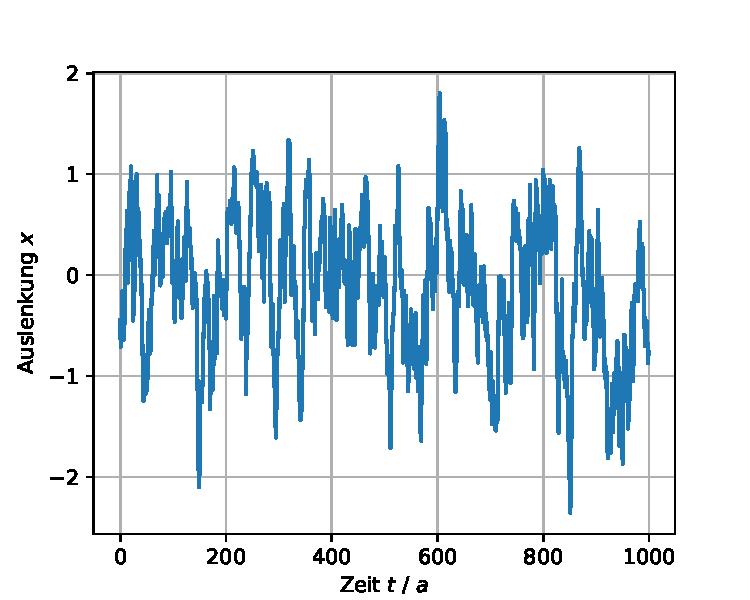
\includegraphics[width=.7\textwidth]{lasttrajectory}
    \caption{Ein Beispiel für eine Trajektorie des harmonischen Oszillators
    nach 10000 Sweeps des Metropolisalgorithmus'.}
    \label{fig:lastTrajectory}
\end{figure}

Um das zuvor Beschriebene etwas besser greifbar zu machen, soll es im Folgenden
kurz anhand des quantenmechanischen harmonischen Oszillators erläutert werden. Die
Wirkung des harmonischen Oszillators lautet nach Anwendung der
Wick-Rotation\footnote{Man bemerke den relativen Faktor $+1$ zwischen kinetischem
und Potentialterm, anders als im Fall mit Minkowski-Raumzeit!}
\[
    S[x] = \int_0^T \dd{t} \left\{ \frac{m}{2} \dot{x}(t)^2
    + \frac{\omega^2}{2} x(t)^2) \right\},
\]
Die Trajektorien $x$ werden einfach als eindimensionales Array gespeichert, der
Einfachheit halber nehmen wir $m=\omega=1$ an. Dann lautet die auf dem Gitter
formulierte, diskretisierte Version der Wirkung
\[
    S[x] = \frac{a}{2} \sum_{i=1}^{N} \left\{\left( \frac{x_i - x_{i-1}}{a} \right)^2
    + x_i^2 \right\}.
\]
Es ist klar, dass für $\Delta S[x'_i, x_i, x]$ nur wenige Terme aus dieser Summe
benötigt werden. In der Simulation wurden insgesamt 10000 Sweeps durchgeführt, wobei
das System \enquote{kalt}, also mit $x_i = 0 \, \forall x_i \in x$ initialisiert wurde.
Eine Trajektorie am Ende dieser 10000 Sweeps ist exemplarisch in Abb.
\ref{fig:lastTrajectory}
dargestellt. Es wird erwartet, dass sich das System nach vielen Iterationen im
Grundzustand befinden wird. Dies lässt sich durch folgende Überlegung motivieren:
Fügt man in den Propagator \eqref{eq:propagator} einen Einheitsoperator, ausgedrückt
durch die Energieeigenzustände, $\mathds{1} = \sum_n \ket{n} \bra{n}$, ein, so
ergibt sich
\begin{equation} \label{eq:groundStateAtLargeT}
    \bra{x_f} e^{-H t} \ket{x_i}
    = \sum_n \bra{x_f} e^{-H t} \ket{n} \braket{n}{x_i}
    = \sum_n e^{-E_n t} \braket{x_f}{n} \braket{n}{x_i}
    \xrightarrow{t \gg 1} e^{-E_0 t} \braket{x_f}{0} \braket{0}{x_i}.
\end{equation}
Für große $t$, d.\,h. hier nach vielen Iterationen, sollte das System im niedrigst
liegenden Energieeigenzustand liegen. Das wollen wir überprüfen, indem wir die
Energie sowie die Wellenfunktion des Zustands aus den Daten der Simulation
extrahieren.

\begin{figure}[htbp]
    \centering
    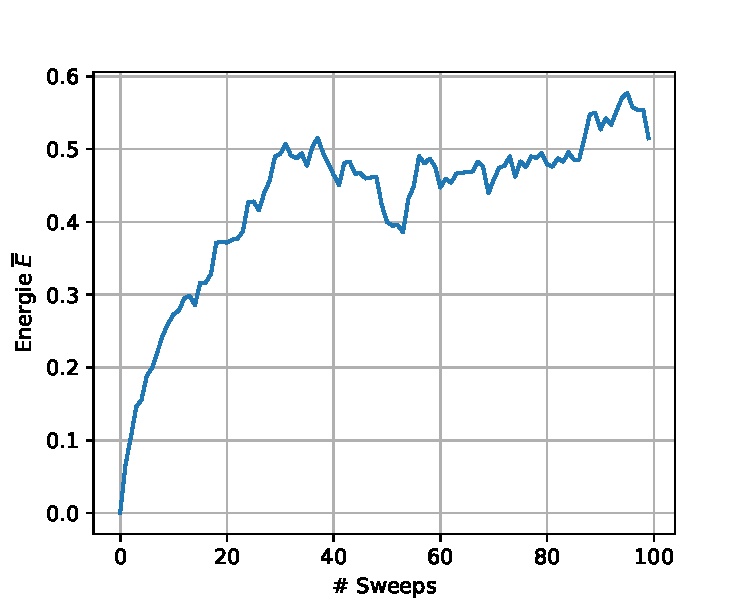
\includegraphics[width=.7\textwidth]{energies}
    \caption{Die gemessenen Energien $\overline{E}$ als Funktion der
    Monte-Carlo-Zeit. Es ist klar eine Konvergenz zu einem Plateau bei $\approx 0.5$
    erkennbar.}
    \label{fig:energies}
\end{figure}

Die Energie ist hier die simplere Sache: Hierfür messen wir zwischen den Sweeps
die Energie
\[
    \overline{E} = \hbar \omega \overline{x^2} = \overline{x^2},
\]
welche der Gesamtwirkung des Systems entspricht\footnote{$x$ ist die Position des
eindimensionalen harmonischen Oszillators. In dieser Rechnung wurde
der Virialsatz miteinbezogen: $T = \frac{1}{2} x V'(x)$. \cite{freedmanCreutz}}.
Das Ergebnis ist
in Abb. \ref{fig:energies} dargestellt: Zunächst ist deutlich sichtbar, wie das System
vom \enquote{kalten} Anfangszustand in den Gleichgewichtszustand konvergiert. Die
Werte zum Berechnen der Grundzustandsenergie nehmen wir ab 1000 Sweeps und
messen nur alle 50 Sweeps, um die Korrelation zwischen den Werten zu verringern.
Wir finden
\[
    \overline{\overline{E}} = 0.491 \pm 0.017,
\]
was den theoretischen Wert $E_0 = \hbar \omega (0 + \frac{1}{2}) = 0.5$
\cite{freedmanCreutz} in den Fehlerbereich miteinschließt. Hierbei wurde die
Unsicherheit auf die Messung durch den Standardfehler abgeschätzt.


\begin{figure}[htbp]
    \centering
    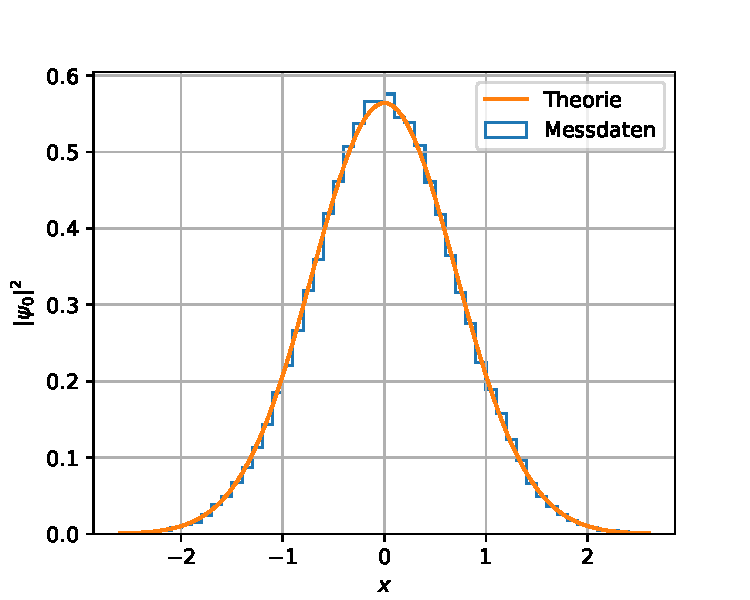
\includegraphics[width=.7\textwidth]{harmonicOscillatorDensity.pdf}
    \caption{Zustandsdichte des Grundzustands des harmonischen Oszillators.}
    \label{fig:harmonicOscDensity}
\end{figure}

Die Grundzustandswellenfunktion $\psi_0$ lässt sich zwar nicht als eine direkte
Observable messen, mittels eines Tricks können wir ihr Betragsquadrat $| \psi_0 |^2$
aber dennoch aus den Daten extrahieren. Hierfür nehmen wir einfach alle Positionen
aus allen Sweeps und stellen sie in einem Histogramm dar. Da $| \psi_0 |^2$ die
Wahrscheinlichkeitsdichte beschreibt, sollte das Histogramm ebendiese Verteilung
widerspiegeln. In Abb. \ref{fig:harmonicOscDensity} ist beides dargestellt, das
erwartete Verhalten ist eingetreten.

\section{Das SU(2)-Eichfeld auf einem Gitter}
\subsection{Yang-Mills}
Hauptbetrachtungsobjekt dieser Arbeit soll das Eichfeld $A_\mu$ der
SU(2)-Eichsymmetrie sein. Der Lagrangian der betrachteten Theorie enthält 
Terme
\[
    \overline{\psi}(x)(i \gamma^\mu \partial_\mu - m) \psi(x),
\]
bei $\psi$ handelt es sich also um ein fermionisches Feld\footnote{Hinzuzufügen
ist, dass es sich hierbei um eine stark vereinfachte Version handelt: In der
Realität wäre noch die Farbladung zu berücksichtigen~\cite{gattringerLang}.}.
Die betrachtete Eichtransformation wirkt auf die Felder dann wie folgt
\cite{gattringerLang}:
\[
    \psi(x) \mapsto \Omega(x) \psi(x), \; \Omega(x) \in \mathrm{SU}(2).
\]
Damit die Theorie eichinvariant wird, soll die Ableitung der Felder genauso
transformieren wie die Felder selbst und dafür muss $\partial_\mu$
durch eine kovariante Ableitung
\[
D_\mu = \partial_\mu + i A_\mu
\]
ersetzt werden. Hier ist $g$ die Kopplungsstärke. Das Eichfeld lässt sich in
seine Farbkomponenten zerlegen \cite{gattringerLang}
\[
    A_\mu = \frac{1}{2} \sum_{a = 1}^3 \tau^a A_\mu^a,
\]
wobei $\tau^a$ die Generatoren der Gruppe SU(2) sind. Im Rahmen dieser Arbeit
seien die Farbindizes stets unterdrückt, für eine explizitere Betrachtung sei
z.\,B. auf das Buch von Gattringer und Lang \cite{gattringerLang} verwiesen.
Als weitere Konvention wurde die Kopplungsstärke $g$ als Faktor in das Feld
absorbiert, daher taucht sie in der kovarianten Ableitung nicht
auf~\cite{gattringerLang}. 

Setzen wir nun als Transformationsverhalten für das Eichfeld
\[
    A_\mu(x) \mapsto \Omega(x) A_\mu(x) \Omega(x)^\dag
    + i \left( \partial_\mu \Omega(x) \right) \Omega(x)^\dag
\]
an \cite{gattringerLang}, so finden wir unter Verwendung von
$\Omega^\dag \Omega = \mathds{1}$
\begin{align*}
    D_\mu(x) \psi(x) \mapsto
    &\left( \partial_\mu + i \Omega(x) A_\mu \Omega(x)^\dag
    - \left( \partial_\mu \Omega(x) \right) \Omega(x)^\dag \right)
    \Omega(x) \psi(x)\\
    = &\left( \partial_\mu \Omega(x) \right) \psi(x)
    + \Omega(x) \partial_\mu \psi(x) + i \Omega(x) A_\mu(x) \psi(x)
    - \left( \partial_\mu \Omega(x) \right) \psi(x) \\
    = &\Omega(x) D_\mu(x) \psi(x).
\end{align*}
So kann also die Eichinvarianz der Theorie erreicht werden.

Die Dynamik des Eichfelds wird typischerweise durch die Yang-Mills-Wirkung
\begin{equation} \label{eq:yang-millsAction}
S[A] = \frac{1}{2 g^2} \int \dd^4{x} \, \mathrm{tr}\,
\left[ F_{\mu \nu}(x) F^{\mu \nu}(x) \right]
\end{equation}
beschrieben. \cite{gattringerLang} Hierbei ist
\[
F_{\mu \nu}(x) = -i [D_\mu(x), D_\nu(x)]
= \partial_\mu A_\nu(x) - \partial_\nu A_\mu(x) + i [A_\mu(x), A_\nu(x)]
\]
der Feldstärketensor. Hier ist die Kopplungskonstante $g$ dann explizit mit
notiert. Zunächst soll nun eine Version dieser Wirkung auf einem Gitter definiert
werden.

\subsection{Wilson}
Um die Integration über alle Dimensionen der Raumzeit zu implementieren,
brauchen wir ein vierdimensionales Gitter. Dieses Gitter habe in Zeitrichtung
eine Ausdehnung von $L_\mathrm{t}$ Gitterpunkten und in die drei Raumrichtungen
jeweils eine Ausdehnung von $L_\mathrm{s}$ Gitterpunkten. Wir verwenden
periodische Randbedingungen: Man kann das Gitter nicht \enquote{verlassen},
sondern läuft immer auf der gegenüberliegenden Seite wieder hinein. Befindet
man sich z.\,B. bei $(L_\mathrm{t}-1,0,0,0)$ und geht einen Schritt in
Zeitrichtung, so befindet man sich danach wieder bei $(0,0,0,0)$. Das Gitter
ist gewissermaßen in jeder Dimension an den Enden zusammengeklebt:
\[
\Lambda = \{0, 1, \dots, L_\mathrm{t}-1\}/(0 \sim L_\mathrm{t}-1)
\times \left( \{0, 1, \dots, L_\mathrm{s}-1 \} / (0 \sim L_\mathrm{s}-1) \right)^3,
\]
es handelt sich also um einen vierdimensionalen, diskretisierten Hypertorus.
Der Abstand der Gitterpunkte sei $a$; als Basis für das Gitter wählen wir die
Vektoren $a_\mu$, die von einem Gitterpunkt auf den nächsten in Richtung $\mu$
zeigen. Sie haben folglich die Länge $a$ und die Basis ist demnach keine
Ortho\emph{normal}basis.

Nun wollen wir unsere Felder auf dem Gitter definieren. Die kanonische
Entscheidung wäre, ihren Definitionsbereich auf das Gitter zu beschränken.
Leider zeigt sich bereits beim fermionischen Feld, dass das so einfach nicht
ist. Die diskretisierte Ableitung ließe sich z.\,B. so umsetzen:
\[
\partial_\mu \psi(x) = \frac{\psi(x + a_\mu) - \psi(x)}{a}.
\]
Betrachten wir dann das Verhalten so einer Ableitung unter der Eichtransformation,
so finden wir
\[
\partial_\mu(x) \psi(x) \mapsto
\frac{\Omega(x + a_\mu) \psi(x + a_\mu) - \Omega(x) \psi(x)}{a}.
\]
Dieses Ergebnis ist insofern problematisch, als dass wir durch die oben
so geschickt eingeführte kovariante Ableitung $D_\mu$ nicht das gewünschte
Transformationsverhalten erreichen können. Das liegt daran, dass hier
$\Omega$ an zwei verschiedenen Orten, $x$ und $x + a_\mu$, verwendet wird. Die
Lösung für dieses durch die Diskretisierung entstandene Problem findet sich in sog.
Paralleltransporten $U_\mu(x) \in \mathrm{SU}(2)$, deren Transformationsverhalten durch
\[
    U_\mu(x) \mapsto \Omega(x) U_\mu(x) \Omega(x + a_\mu)^\dag
\]
definiert ist~\cite{gattringerLang}. Verwenden wir dann die folgende neue kovariante
Ableitung
\[
    \tilde{D}_\mu \psi(x) =
    \frac{U_\mu(x) \psi(x + a_\mu) - \psi(x)}{a},
\]
so erhalten wir wieder das gewünschte Transformationsverhalten
\begin{align*}
    \tilde{D}_\mu \psi(x) \mapsto
    &\frac{\Omega (x) U_\mu(x)
    \overbrace{\Omega(x + a_\mu)^\dag \Omega(x + a_\mu)}^{= \mathds{1}}
    \psi(x + a_\mu) - \Omega(x) \psi(x)}{a} \\
    = & \Omega(x) \tilde{D}_\mu \psi(x).
\end{align*}
Die Paralleltransporte verdienen noch etwas Aufmerksamkeit: $U_\mu(x)$ kann als
\enquote{Zeiger} von $x$ nach $x + a_\mu$ interpretiert werden. Umgekehrt zeigt
$U_\mu(x)^\dag$ von $x + a_\mu$ auf $x$. \cite{urbachCPscript} Um die Verbindung
zum Eichfeld $A_\mu(x)$ herzustellen, reicht ein Blick auf ihre genaue
mathematische Definition \cite{gattringerLang}
\[
    U_\mu(x) = P \exp(i \int_\gamma \dd{s} A_\mu),
\]
hier ist $\gamma$ ein Pfad, der $x$ mit $x + a_\mu$ verbindet. Wenn man die
direkte Verbindungslinie für $\gamma$ annimmt und das Integral nun zu erster
Ordnung in $a$ auf dem Gitter ausführt, so findet man \cite{gattringerLang}
\begin{equation} \label{eq:parallelTransportexpA}
    U_\mu(x) = \exp(i a A_\mu(x)).
\end{equation}
Dieser Zusammenhang wird im Folgenden nützlich sein bei der Betrachtung der
Wilson-Wirkung, welche das Verhalten des Eichfelds auf einem Gitter beschreibt
\cite{urbachCPscript}:
\begin{equation} \label{eq:wilsonAction}
    S_\text{Wilson} = \frac{\beta}{2} \sum_{x \in \Lambda} \sum_{\mu < \nu}
    \text{Re} \; \text{tr} \left[\mathds{1} - U_{\mu \nu}(x) \right].
\end{equation}
Üblicherweise wird in dieser Formulierung die inverse Kopplung
$\beta = \frac{2 N_\text{c}}{g^2} = \frac{4}{g^2}$ verwendet. Was ist hier 
$U_{\mu \nu}$? Es handelt es sich um den kleinstmöglichen geschlossenen Ring von
Paralleltransporten \cite{urbachCPscript}
\[
    U_{\mu \nu}(x) = U_\mu(x) U_\nu(x + a_\mu) U_\mu(x + a_\nu)^\dag U_\nu(x)^\dag,
\]
der auch \emph{Plaquette} genannt wird. Man sieht leicht, dass die Spur\footnote{In
dieser Arbeit sind alle betrachteten Observablen $X$ die Spur einer Funktion 
von Paralleltransporten $X = \text{tr} \, Y$. Deswegen ist stets die Spur
$\text{tr} \, Y$ gemeint, auch wenn nur von $Y$ als Observable gesprochen wird.
Die Spur ist immer notwendig, um mit ihrer zyklischen Eigenschaft die Eichinvarianz
der Observablen zu erreichen.}
dieser Plaquette (wie die aller geschlossenen Ringe von Paralleltransporten)
eichinvariant ist, was auch die formulierte Wilson-Wirkung eichinvariant macht.
Nun wollen wir zeigen, dass die Wilson-Wirkung für kleine Gitterabstände $a$ wieder
in die Yang-Mills-Wirkung \eqref{eq:yang-millsAction} übergeht.

Dazu betrachten wir zunächst die Plaquette im Rahmen des oben gefundenen
exponentiellen Ausdrucks für die Paralleltransporte \eqref{eq:parallelTransportexpA}:
\begin{align*}
    U_{\mu \nu}(x) =
    &\exp(i a A_\mu(x)) \exp(i a A_\nu(x + a_\mu))
    \exp(-i a A_\mu(x + a_\nu)) \exp(-i a A_\nu(x)) \\
    = &\exp \left\{ i a \left(A_\mu(x)
    + A_\nu(x + a_\mu) - A_\mu(x + a_\nu)
    - A_\nu(x) \right) \right. \\
    &+ \frac{i a^2}{2} \left(-[A_\mu(x), A_\nu(x + a_\mu)]
    + [A_\mu(x), A_\mu(x + a_\nu)] \right. \\
    &+ [A_\mu(x), A_\nu(x)] + [A_\nu(x + a_\mu), A_\mu(x + a_\nu)] \\
    &+ \left. \left. [A_\nu(x + a_\mu), A_\nu(x)] \right) + \mathcal{O}(a^3) \right\} \\
    = &\exp{i a \cdot 0 + i a^2 \left(\partial_\mu A_\nu(x)
    -\partial_\nu A_\mu(x) + i [A_\mu(x), A_\nu(x)] \right) + \mathcal{O}(a^3)} \\
    = &\exp(i a^2 F_{\mu \nu}(x) + \mathcal{O}(a^3)).
\end{align*}
Hierbei wurde eine Version der Baker-Campbell-Hausdorff-Regel \cite{gattringerLang}
\[
    e^A e^B = e^{A + B + \frac{1}{2} [A, B] + \cdots}
\]
verwendet. Im zweiten Schritt wurden die Felder um $x$ entwickelt, also z.\,B.
\[
    A_\mu(x + a_\nu) = A_\mu(x) + a \partial_\nu A_\mu(x) + \mathcal{O}(a^2).
\]
Setzen wir das gefundene Ergebnis in die Wilson-Wirkung
\eqref{eq:wilsonAction} ein, so erhalten wir unter Berücksichtigung der
Antisymmetrie des Feldstärketensors \cite{gattringerLang}
\begin{align*}
    S_\text{Wilson} &= \frac{\beta}{2} \sum_{x \in \Lambda} \sum_{\mu < \nu}
    \text{tr} \left[\mathds{1} - \mathds{1}
    + \frac{1}{2} (a^2 F_{\mu \nu}(x))^2
    + \mathcal{O}(a^8) \right] \\
    &= \frac{a^4}{2 g^2} \sum_{x \in \Lambda} \text{tr} \left[ \sum_{\mu, \nu}
    (F_{\mu \nu}(x))^2 \right] + \mathcal{O}(a^8).
\end{align*}
Die Wilson-Wirkung bietet also eine ordentliche Annäherung an die im Kontinuum
formulierte Yang-Mills-Wirkung und kann für unsere Zwecke verwendet werden.

\subsection{Haar}
Für die Berechnung von Erwartungswerten auf dem Gitter wird ein Integrationsmaß
für die Paralleltransporte benötigt. Die naheliegende Wahl wäre \cite{gattringerLang}
\[
    \mathscr{D}[\mathcal{U}] = \prod_{x \in \Lambda} \prod_{\mu = 0}^3 \dd{U_\mu(x)}.
\]
Hier ist $\mathcal{U} = \{U_\mu(x) \, | x \in \Lambda, \mu \in \{0,1,2,3\}\}$ die
Menge aller Paralleltransporte auf dem Gitter. Hiermit finden wir also z.\,B.
\[
    Z = \int \mathscr{D}[\mathcal{U}] e^{-S_\text{Wilson}[\mathcal{U}]}.
\]
Auch für diese Größe wollen wir die Eigenschaft der Eichinvarianz ansetzen können,
damit die schlussendlich berechneten Erwartungswerte ebenfalls eichinvariant sind.
Da die Wilson-Wirkung bereits eichinvariant ist, muss also folgendes gelten:
\[
    \dd{U'_\mu(x)} = \dd{\left( \Omega(x) U_\mu(x) \Omega(x + a_\mu)^\dag \right)}
    \overset{!}{=} \dd{U_\mu(x)}.
\]
Der perfekte Kandidat für dieses Problem ist das sog. Haar-Maß, welches für Elemente
einer Gruppe $U, V \in G$ definiert ist und folgende Bedingungen erfüllen muss
\cite{gattringerLang}:
\[
    \dd{(U V)} = \dd{(V U)} = \dd{U}, \; \int \dd{U} = 1.
\]
Für eine etwas detailliertere Diskussion dieses Themas sei auf das Buch von
Gattringer und Lang \cite{gattringerLang} verwiesen, hier soll uns genügen, dass
das Integrationsmaß die genannten Bedingungen erfüllt und so unsere Erwartungswerte
eichinvariant macht.

\subsection{Wilson und Metropolis} \label{sec:wilsonMetropolis}
Um den Metropolisalgorithmus auf dem Gitter umsetzen zu können, fehlt uns noch eine
effiziente Methode, um $\Delta S$ zu berechnen. Es ist einleuchtend, dass die durch
die Veränderung eines einzelnen Paralleltransports $U_\mu(x)$ modifizierten Plaquettes
ebenjene sind, an denen $U_\mu(x)$ als \enquote{Kante} beteiligt ist. Je Ebene
$(\mu, \nu)$ in der Raumzeit gibt es hiervon zwei -- \enquote{oberhalb} und
\enquote{unterhalb} von $U_\mu(x)$. Wir finden also
\begin{align*}
    \Delta S &= -\frac{\beta}{2} \sum_{\nu \neq \mu} \mathrm{tr} \left[ \right.
        U'_{\mu \nu}(x) - U_{\mu \nu}(x)
        + U'_{\mu \nu}(x - a_\nu) - U_{\mu \nu}(x - a_\nu) \left. \right] \\
    &= -\frac{\beta}{2} \sum_{\nu \neq \mu} \mathrm{tr} \left[ \right.
        U'_{\mu \nu}(x) - U_{\mu \nu}(x)
        + (U'_{\mu \nu}(x - a_\nu) - U_{\mu \nu}(x - a_\nu))^\dag \left. \right] \\
    &= -\frac{\beta}{2} \sum_{\nu \neq \mu} \mathrm{tr} \left[ \right.
       (U'_\mu(x) - U_\mu(x)) U_\nu(x + a_\mu) U_\mu(x + a_\nu)^\dag U_\nu(x)^\dag \\
    & \qquad \qquad + U_\nu(x - a_\nu) (U'_\mu(x) - U_\mu(x))
    U_\nu(x + a_\mu - a_\nu)^\dag U_\mu(x - a_\nu)^\dag \left. \right] \\
    &= -\frac{\beta}{2} (U'_\mu(x) - U_\mu(x)) \sum_{\nu \neq \mu}
    \text{tr} \left[ \right. U_\nu(x + a_\mu) U_\mu(x + a_\nu)^\dag U_\nu(x)^\dag \\
    & \qquad \qquad \qquad  \qquad \underbrace{\qquad+ U_\nu(x + a_\mu - a_\nu)^\dag
    U_\mu(x - a_\nu)^\dag
    U_\nu(x - a_\nu) \left. \right]}_{\eqqcolon K_{\mu \nu}(x)}.
\end{align*}
Hier wurde im zweiten Schritt
$\text{tr} \, U = \text{tr} \, U^\dag \; \forall U \in \text{SU}(2)$
und im dritten Schritt die Zyklizität der Spur verwendet. Die Größe $K_{\mu \nu}(x)$
wird \emph{staple} genannt. Wie zuvor angedeutet, muss also für die Berechnung von
$\Delta S [U'_\mu(x), U_\mu(x), \mathcal{U}]$ nicht das gesamte Gitter berücksichtigt
werden, es
genügt die Betrachtung der $3 \cdot 6 = 18$ umliegenden Paralleltransporte.


\subsection{Das statische Potential und Wilson-Loops} \label{sec:thWilsonLoops}
Eine wichtige Observable auf dem Gitter sind sog. Wilson-Loops, die geschlossene
Ringe von Paralleltransporten darstellen. Im einfachsten Fall kann man sie sich
als Rechteck vorstellen:
\[
    W(x, \mu, \nu, m, n) = \text{tr} \left[ L(x, \mu, m)
    \cdot L(x + m a_\mu, \nu, n) \cdot L(x + n a_\nu, \mu, m)^\dag
    \cdot L(x, \nu, n)^\dag \right],
\]
\[
    L(x, \mu, m) = \prod_{i=0}^{m-1} U_\mu(x + i a_\mu)
\]
Man erkennt gut, dass es sich hierbei um die Verallgemeinerung der zuvor besprochenen
Plaquette $U_{\mu \nu}(x)$ handelt.
Im folgenden soll motiviert werden, dass sich aus dem Erwartungswert
$\langle W(0, i, l_\text{t}, l_\text{s}) \rangle =: \langle W(r,t)\rangle$
das Potential zweier unendlich schwerer, immobiler (\enquote{statischer}) Quarks mit
Abstand $r = l_\text{s} a$ extrahieren lässt.

Ausgangspunkt ist die Überlegung \eqref{eq:groundStateAtLargeT}, welche wir beim
harmonischen Oszillator angestellt haben: Für große Zeiten $t$ wird ein
physikalisches System im Rahmen des Feynman'schen Pfadintegralformalismus stets
auf den mit dem Grundzustand überlappenden Zustand übergehen. Nun ist also das Ziel,
einen Quark-Antiquark-Paar-Zustand zu erzeugen, der bei konstantem Ort durch die
Zeit propagiert und dann wieder annihiliert wird.

Die naheliegende Entscheidung liegt in einer Kombination des Propagators eines
unendlich schweren Quarks an einer konstanten Position $x$ \cite{latticeQCDforNovices}
\[
    G_\infty(t, \vec{x}) = U_0(t-a, \vec{x})^\dag U_0(t-2a, \vec{x})^\dag
    \dots U_0(0, \vec{x})^\dag
\]
mit dem eines unendlich schweren Antiquarks, $G_\infty(t, \vec{y})^\dag$. Hier haben
wir bereits zwei \enquote{Kanten} des späteren Wilson-Loops. Um das Konstrukt
eichinvariant zu machen, fügen wir zwei weitere Kanten hinzu, die $(0,\vec{x})$
und $(0,\vec{y})$ bzw. $(t,\vec{x})$ und $(t,\vec{y})$
verbinden.\footnote{Hier sei hinzugefügt, dass diese beiden Kanten sich jederzeit
durch sog. \emph{gauge fixing} wieder \enquote{entfernen} lassen, vgl. hierfür z.\,B. 
\cite{gattringerLang}.} So haben wir die zuvor definierten Wilson-Loops wiedergefunden
und finden für ihren Erwartungswert \cite{loopsStaticPotRothe}
\begin{equation} \label{eq:wilsonStaticPot}
    \langle W(r,t) \rangle = C \cdot e^{-t V(r)}.
\end{equation}
Im weiteren Verlauf dieser Arbeit werden wir also Wilson-Loops verschiedener Maße
$\overline{W(r,t)}$ messen und durch Anpassungen von exponentiellen Modellen an die
gewonnenen Daten das statische Potential extrahieren. Es ist auch möglich, sog.
\emph{nichtplanare} Wilson-Loops zu vermessen, also solche, die nicht der oben
benannten, rechteckigen Form entsprechen. So ist es möglich, auch nichtganzzahlige
Abstände $r$ zu vermessen.

Die hier vorgenommene Diskussion dieser Observablen erhebt keinerlei Anspruch auf
Vollständigkeit oder Rigorosität. Eine in dieser Hinsicht bessere Betrachtung ist
im Buch von Rothe \cite{loopsStaticPotRothe} zu finden. 

% !TEX root = mythesis.tex

%==============================================================================
\chapter{Methodik und Implementation}
\label{sec:implementation}
%==============================================================================

\section{SU(2)-Matrizen} \label{sec:su2matrix}
Nachdem die theoretischen Grundlagen gelegt wurden, kann mit der Implementation
des Algorithmus begonnen werden. Zunächst wird hierfür eine numerische Darstellung
von SU(2)-Matrizen benötigt. Die hier verwendete Form ist an die von Urbach und
Petschlies \cite{urbachCPscript} angelehnt. Aus der Definition von unitären Matrizen
\[
    U^\dag U = U U^\dag = \mathds{1}
\]
lässt sich ableiten, dass sich jede unitäre $2 \times 2$-Matrix in der Form
\[
U =
\begin{pmatrix}
    a    & b   \\
    -b^* & a^* \\
\end{pmatrix},
\; a, b \in {C}, \; |a|^2 + |b|^2 = 1.
\]
darstellen lässt~\cite{urbachCPscript}.

Die Klasse speichert also lediglich die Einträge der oberen Zeile einer jeden Matrix.
Man kann zeigen, dass sich Matrixmultiplikation im Rahmen dieser Darstellung wie
folgt umsetzen lässt~\cite{urbachCPscript}:
\[
    (a_1, b_1) \cdot (a_2, b_2) = (a_1 b_2 - b_1 b_2^*, a_1 b_2 + b_1 a_2^*).
\]
Die weiteren Matrixoperationen ergeben sich trivial aus der verwendeten Form:
\begin{align*}
    (a_1, b_1) + (a_2, b_2) &= (a_1 + a_2, b_1 + b_2), \\
    (a, b)^\dag &= (a^*, -b), \\
    \text{tr}~(a, b) &= 2 \, \text{Re} \, a.
\end{align*}
Aufgrund der endlichen Präzision der verwendeten Datentypen muss für eine betrachtete
Matrix $U$ hin und wieder $\text{det} \, U = 1$ forciert werden. Die geschieht durch
\cite{urbachCPscript}
\[
    (a, b) \mapsto \left(\frac{a}{\sqrt{|a|^2 + |b|^2}},
    \frac{b}{\sqrt{|a|^2 + |b|^2}}\right).
\]

\section{Zufällige SU(2)-Matrizen} \label{sec:randomSU2}
Eine Herausforderung bildet die Generierung zufälliger Paralleltransporte $U'_\mu(x)$,
die, wie in Abschnitt~\ref{sec:metropolis} erwähnt, \enquote{nah} an $U_\mu(x)$ liegen
sollen. Hierzu nutzen wir, dass SU(2) isomorph zur Sphäre $S^3$ ist vermöge des
Isomorphismus \cite{urbachCPscript}
\begin{align*}
    \phi: S^3 &\rightarrow \mathrm{SU}(2),\\
    (x^0, \vec{x}) &\mapsto x^0 \mathds{1} + i \vec{x} \cdot \vec{\sigma}.
\end{align*}
Hier sind $\{\sigma^i\}_{i \in \{1,2,3\}}$ die Paulimatrizen. Für die Punkte auf $S^3$
verwenden wir Kugelkoordinaten
\[
    \begin{pmatrix}
    x^0 \\
    x^1 \\
    x^2 \\
    x^3
    \end{pmatrix}
    =
    \begin{pmatrix}
    \cos(\chi) \sin(\vartheta) \cos(\varphi) \\
    \sin(\chi) \sin(\vartheta) \cos(\varphi) \\
    \sin(\chi) \sin(\vartheta) \sin(\varphi) \\
    \sin(\chi) \cos(\vartheta)
    \end{pmatrix}.
\]
Folgende Zufallszahlen werden uniform generiert:
\begin{align*}
    \chi &\in (0, 2 \pi \cdot \delta),\\
    \varphi &\in (0, 2 \pi),\\
    \cos(\vartheta) &\in (-1,1).
\end{align*}
Hier kann $\delta > 0$ beliebig klein gewählt werden, sodass die resultierende
Matrix
\begin{align*}
    R &= (x^0 + i x^3, x^2 + i x^1) \\
    &= (\cos(\chi) + i \sin(\chi) \cos(\vartheta),
    \sin(\chi) \sin(\vartheta) \sin(\varphi) + i \sin(\chi) \sin(\vartheta) \cos(\varphi))
\end{align*}
nah an $\mathds{1}$ liegt\footnote{Es sei erwähnt, dass selbst bei
$\delta = 1$ die generierten Punkte nicht isotrop auf $S^3$ verteilt sein werden.
Hierfür müssten die Koordinaten anders generiert werden. Der Algorithmus ist aber
so gestaltet, dass $\vec{x}$ isotrop auf $S^2$ verteilt sind (daher die Generierung
von $\cos(\vartheta) \in (-1,1)$). Da $\delta$ stets klein gewählt wird, genügt
dies für unsere Zwecke.}. Dann kann
für ein gegebenes $U_\mu(x)$ der neue Kandidat durch
\[
    U'_\mu(x) = R \cdot U_\mu(x)
\]
erzeugt werden.

\section{Implementierung des Algorithmus' sowie der Observablen}
Der beschriebene Algorithmus wurde in C++ implementiert, der Programmcode ist auf
Github\footnote{\url{https://github.com/s6hevonc/bachelorarbeit}} einsehbar. Hier soll nur eine kurze Auflistung der wichtigsten Klassen
und Funktionen folgen, die Details lassen sich in den Header Files nachlesen.

Die Klasse \texttt{SU2matrix} ist die Repräsentation unitärer $2 \times 2$-Matrizen,
wie sie in Abschnitt \ref{sec:su2matrix} beschrieben ist. Es wird jeweils die obere
Reihe der Matrix mit zwei Einträgen vom Typ \texttt{std::complex<double>} gespeichert.
Die Klasse enthält eine Methode \texttt{renormalise()}, welche die Forcierung der
Determinante auf 1 umsetzt sowie eine Methode \texttt{dagger()} für die hermitesche
Adjunktion. Für die Addition und Multiplikation wurden die entsprechenden Operatoren
\emph{überladen}, d.\,h. für zwei Instanzen \texttt{A} und \texttt{B} der Klasse kann 
ihre Summe resp. ihr Produkt durch \texttt{A + B} resp. \texttt{A * B} berechnet
werden. Schließlich gibt es eine Funktion \texttt{randomSU2}, die eine zufällige
SU(2)-Matrix wie in Abschnitt \ref{sec:randomSU2} beschrieben generiert; sie nimmt
$\delta$ für die Stärke der \enquote{Abweichung} von $\mathds{1}$ als Argument entgegen.

Die zweite Klasse heißt \texttt{Gaugeconfig}. Eine Instanz \texttt{U} beschreibt den
Zustand des Eichfeldes in Form der Paralleltransporter auf einem geg. Gitter, im
Wesentlichen handelt es sich also um ein fünfdimensionales Array der Maße
$L_\text{t} \times L_\text{s} \times L_\text{s} \times L_\text{s} \times 4$.
Die 4 am Ende rührt daher, dass je Gitterpunkt $x$ vier Paralleltransporter
$U_\mu(x)$ vorliegen, einer in jede Raumzeitrichtung. Wichtigste Methode der Klasse
ist die Überladung des \texttt{()}-Operators. Konkret kann auf $U_\mu(x)$ mit
\texttt{U(x, mu)} zugegriffen werden. Hier sind auch direkt die periodischen
Randbedingungen implementiert: \texttt{x} ist ein \texttt{std::vector<long int>},
der auch negative Einträge haben kann. Zugehörig zu \texttt{Gaugeconfig} ist noch
die Funktion \texttt{hotStart}, welche zu gegebenen Gittermaßen $L_\text{t}$ und
$L_\text{s}$ und dem Parameter $\delta$ eine Konfiguration \texttt{U} zurückgibt,
welche an jeden Gitterpunkt zufällig generierte SU(2)-Matrizen enthält.

Die für den Metropolisalgorithmus notwendigen Staples (vgl. Abschn.
\ref{sec:wilsonMetropolis} sind mittles der Funktion \texttt{getStaple} zu berechnen.
Der fertige Algorithmus ist dann in der Funktion \texttt{sweep} implementiert, welche
eine einzelne Iterationen auf einer gegebenen \texttt{Gaugeconfig} durchführt.
Hierbei kann $\delta$ für die Zufallsgenerierung sowie die Anzahl der Iterationen
je Paralleltransport spezifiziert werden.

Für die Observablen existiert zunächst die Funktion \texttt{getPlaquette}, welche
die Plaquette ausgehend von einem geg. Gitterpunkt $x$ zurückgibt. Die Funktion
\texttt{gaugeEnergy} berechnet die gesamte Wirkung des Gitters. Weiterhin gibt
die Funktion \texttt{getPlanarLoop} den Wert eines planaren Wilson-Loops zurück.
Schließlich finden sich in \texttt{getSqrt2Loop}, \texttt{getSqrt3Loop} etc.
einzelne Funktionen, die nichtplanare Wilson-Loops vermessen. So ist es möglich,
auch nicht ganzzahlige $r$ für den Abstand des Quark-Antiquark-Paares zu betrachten.


\section{Parameter und Ablauf der durchgeführten Simulationen}
Um einen Überblick über den Ablauf der Simulation zu bieten, ist in Listing
\ref{lst:main} eine exemplarische \texttt{main}-Funktion nachzulesen.

\begin{lstlisting}[language=C++,float,caption=Ein Beispiel für main.cpp,label=lst:main]
int main()
{
    // for random number genration:
    std::random_device rd {}; // to generate the seed for...
    std::mt19937 engine { rd() }; // Mersenne twister generator

    // lattice parameters
    const std::size_t timeSize { 10 };
    const std::size_t spaceSize { 10 };

    // initial configuration:
    Gaugeconfig U { hotStart(timeSize, spaceSize, engine, 0.) };

    // sweep parameters:
    const double beta { 2.3 };
    const double delta { .1 };
    const std::size_t numberOfSweeps { 10 };
    const std::size_t iterationsPerSight { 10 };

    // to save observables:
    const std::string dataDir { "../data/" };
    const std::string filename { "wilsonsqrt.txt" };
    std::vector<double> results;

    std::cout << "warming up..." << std::endl;
    for (std::size_t i {0}; i < 10; i++)
    {
        sweep(U, beta, delta, iterationsPerSight, engine);
    }

    std::cout << "performing " << numberOfSweeps << " sweeps..." << std::endl;

// define merge behaviour for std::vector:
#pragma omp declare reduction (merge : std::vector<double> : omp_out.insert(omp_out.end(), omp_in.begin(), omp_in.end()))
// parallelised loop: the results are 2 b merged, the engine has to be
// shared over all threads to obtain uncorrelated data, use two threads
#pragma omp parallel for reduction(merge: results), shared(engine), num_threads(2)
    for (std::size_t i=0; i < numberOfSweeps; i++)
    {
        results.push_back(getSqrt2Loop(U, 2));

        for (size_t j = 0; j < 5; j++)
        {
            sweep(U, beta, delta, iterationsPerSight, engine);
        }
    }
    std::cout << "zero if writing successful: ";
    std::cout << write_2d(results, dataDir + filename, ',') << '\n';
    return 0;
}
\end{lstlisting}

Als Erstes werden alle wichtigen Variablen deklariert und initialisiert. Bei
\texttt{std::mt19937} handelt es sich um die C++-Standardimplementation eines
Mersenne-Twister-Generators für Pseudozufallszahlen. Die Messungen werden auf
einem Gitter der Maße $(L_\text{t}, L_\text{s}) = (10,10)$ durchgeführt, welches
zunächst kalt, also mit
$\delta = 0 \rightarrow U_\mu(x) = \mathds{1} \forall x \forall \mu$
initialisiert wird. Als Nächtes werden die
Parameter für die einzelnen Sweeps ($\beta = 2.3, \delta = 0.1$) sowie die
Zahl der Hits je Paralleltransport sowie die Gesamtzahl der Iterationen
festgelegt. Außerdem wird die Speicherung der Messwerte vorbereitet.

Nachdem das Gitter zunächst thermalisiert wird, kann die Messphase beginnen.
Der eigentliche Messvorgang wird, um das Verfahren zu
beschleunigen, mit \texttt{fopenmp} auf mehreren Kernen durchgeführt. Konkret wird
die Schleife mit den Messungen mit dem Befehl in Zeile 37 parallelisiert.
\texttt{reduction(merge: results)} bedeutet, dass die Ergebnisse aus allen Threads
am Ende im Array \texttt{results} zusammen gespeichert werden sollen. Außerdem
ist es wichtig, dass alle Threads
auf die \texttt{engine}, die Instanz des Zufallsgenerators, \emph{gleichzeitig}
zugreifen können: Standardmäßig würde jeder Thread seine eigene Instanz erhalten,
dann wären aber alle in den einzelnen Threads generierten Pseudozufallszahlen gleich
und die resultierenden Daten korreliert. \texttt{num\_threads} spezifiziert die
Anzahl der Threads. Zwischen jeder Messungen werden je fünf Sweeps
durchgeführt, um Korrelation zwischen den Daten zu verringern.

Nach Ablauf der Messphase werden die Daten schließlich noch gespeichert, um sie
danach auswerten zu können. Für alle im folgenden Kapitel diskutierten Daten sind
die Messwerte im Anhang \ref{sec:params} zu finden.

% !TEX root = mythesis.tex

%==============================================================================
\chapter{Auswertung}
\label{sec:auswertung}
%==============================================================================

Nachdem die Simulationen fertiggestellt wurden, sollen hier die gewonnenen Daten
ausgewertet werden, mit der Motivation am Ende das statische Potential des
Quark-Antiquark-Paares zu extrahieren.

\section{Energie und durchschnittliche Plaquette}
Um zunächst ein Gefühl für die Thermalisierung (also das Erreichen des
Gleichgewichtszustands) des Gitters zu bekommen, wurde zwischen den Sweeps zunächst
die Gesamtenergie
\[
    E = \sum_{x \in \Lambda} \sum_{\mu < \nu} \text{Re} \; \text{tr}~U_{\mu \nu}(x)
\]
vermessen, woraus sich auch die durchschnittliche Plaquette
\[
    P = \frac{E}{6 L_t L_s^3 N_\mathrm{c}}
\]
berechnen lässt. Das Ergebnis ist in Abhängigkeit von der Sweepzahl in Abb.
\ref{fig:avgPlaquette} dargestellt. Wie man erkennen kann, wurde das System kalt, d.\,h.
mit $U_\mu(x) = \mathds{1} \forall U_\mu(x) \in \mathcal{U}$ initialisiert, daher
beginnen die Werte bei $P = 1$. In unter 20 Sweeps konvergiert das System dann zu
einem stabilen Plateau. Nun kann der Erwartungswert von $P$ approximiert werden.
Dazu wird wie beim harmonischen Oszillator das arithmetische Mittel und der
Standardfehler von vielen Messwerten von $P$ gebildet. Hier wurden insgesamt
10000 Sweeps durchgeführt. Für $\beta = 1$ erhalten wir
\[
    \overline{P} = 0.24308 \pm 0.00010.
\]
Dieser Wert allein ermöglicht zwar den Vergleich mit vorherigen Simulationen, bietet
allein aber wenig Einblicke in die Physik. Dazu bieten erst die Wilson-Loops
mehr Gelgenheit.

\begin{figure}[htbp]
    \centering
    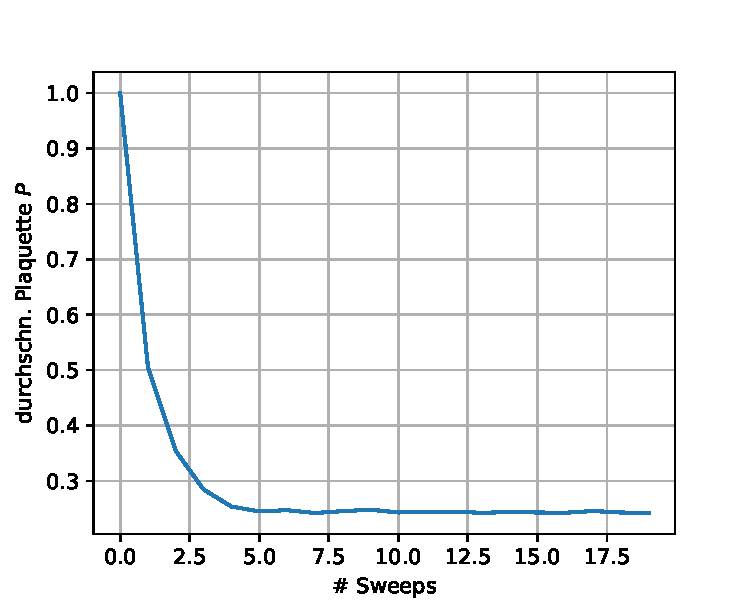
\includegraphics[width=.7\textwidth]{avgPlaquette}
    \caption{Die durchschnittliche Plaquette eines $16 \times 8^3$-Gitters bei
    $\beta = 1$ als Funktion der Iterationszahl: Nach ca. 5 Sweeps scheint das System
    bereits einen Gleichgewichtszustand zu erreichen.}
    \label{fig:avgPlaquette}
\end{figure}

\section{Vermessen von Wilson-Loops verschiedener Größe}

\begin{figure}[htbp]
    \centering
    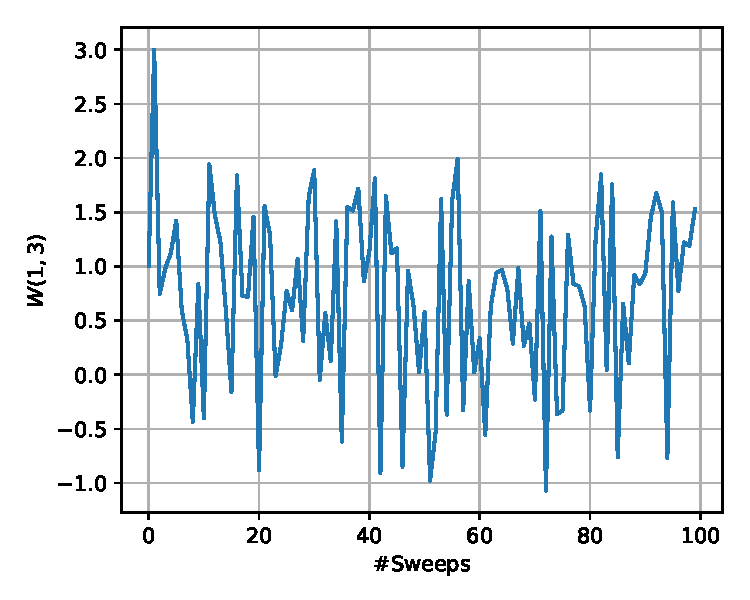
\includegraphics[width=.4\textwidth]{1x3loop}
    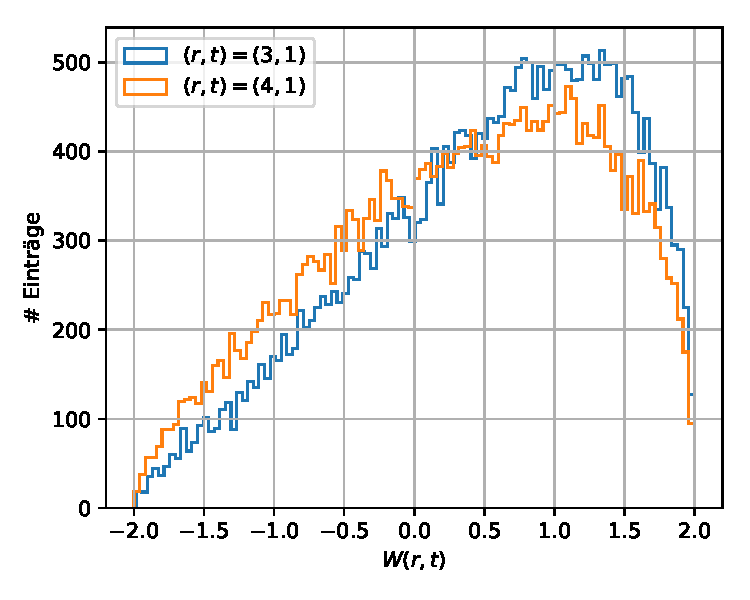
\includegraphics[width=.4\textwidth]{1x3and4histogram}
    \caption{Links: Alle Messwerte eines $1 \times 3$-Wilson-Loops. Rechts:
    Verteilung relevanter Messwerte (nach Equilibrierung alle 5 sweeps gemessen).}
    \label{fig:singleLoops}
\end{figure}

Als Nächstes wurden also planare und nicht-planare Wilson-Loops, also rechteckigen
geschlossenen Ringen von Paralleltransporten betrachtet. Zunächst
wurden Loops wie in Abschn. \ref{sec:thWilsonLoops} definiert zwischen den Sweeps
vermessen. Als Bsp. sind die Messwerte für einen $1 \times 3$-Loop als Funktion der
Sweepzahl in Abb. \ref{fig:singleLoops} dargestellt. Zuerst fällt auf, dass die
Messwerte sehr stark zwischen den Werten $\pm 2$ fluktuieren. Deswegen sind viele
Messwerte zur zuverlässigen Bestimmung des Erwartungswertes notwendig. In
\ref{fig:singleLoops} ist die Verteilung der Messwerte
für zweimal 29800 Messungen dargestellt. Wieder ist zu erkennen, dass die Verteilung
sehr \enquote{breit} ist, und das insbes. für die Unterscheidung der verschiedenen
Messungen viele Messungen notwendig sind, um den Standardfehler auf $\overline{W(r,t)}$
entsprechend zu drücken. In diesem konkreten Fall wurde
\[
    \overline{W(3,1)} = 0.4984 \pm 0.0030, \;
    \overline{W(4,1)} = 0.3270 \pm 0.0032
\]
berechnet. Bemerkenswert ist, dass der Standardfehler in diesem Bsp. und bei allen
Messungen (unabhängig von der Größe der Schätzer) ungefähr gleich groß ist. Dies
ist vermutlich auf die Ähnlichkeit der Verteilung (und somit der Standardabweichung)
und der gleichen Anzahl von Samples zurückzuführen. (Der Standardfehler skaliert mit
$\frac{\sigma}{\sqrt{N}}$.)

\section{Extrahierung der Werte für das statische Potential}

\begin{figure}[htbp]
    \centering
    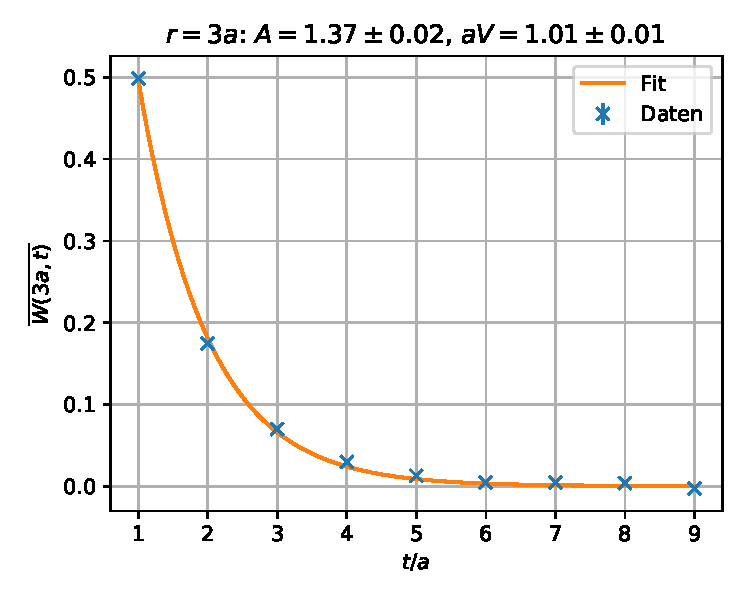
\includegraphics[width=.7\textwidth]{loopResultsBeta23r3.pdf}
    \caption{Beispiel für Wilson-Loop-Messwerte zur Bestimmung des statischen
    Potentials für $r = 3a$. Verwendetes Modell:
    $\overline{W(3a,t)} = A \cdot \exp(-aV t/a)$.}
    \label{fig:loopResultr3}
\end{figure}

Grundlage für die Berechnung des Wertes des statischen Potentials für ein festes
$r$ bietet die Relation \eqref{eq:wilsonStaticPot}. Ziel ist, aus den Daten eine
Abhängigkeit $aV(r)$ zu gewinnen. Zunächst wurde also der
Erwartungswert $\overline{W(r,t)}$ in Abhängigkeit von $t$ betrachtet
Abb. \ref{fig:loopResultr3} exemplarisch für $r = 3a$ dargestellt ist. Dies sollte
eine abklingende Exponentialkurve liefern, deren Exponentialkoeffizient dann dem
statischen Potential bei einem Abstand $r=3a$ entspricht. Der exponentielle
Zusammenhang ist klar erkennbar, ein Fit liefert den gewünschten Parameter
$a V(r)$. ($t$ ist natürlich nur bis auf die Gitterkonstante $a$ bestimmt.) Es
fällt aber auch auf, dass die Messwerte bei größeren $t$ nicht mehr allzu klar
dem exponentiellen Zusammenhang folgen. Natürlich macht sich die Tatsache, dass
der statistische Fehler immer ungefähr gleich groß ist, besonders bei kleinen
Messwerten bemerkbar.

\section{Confinement?}

\begin{figure}[htbp]
    \centering
    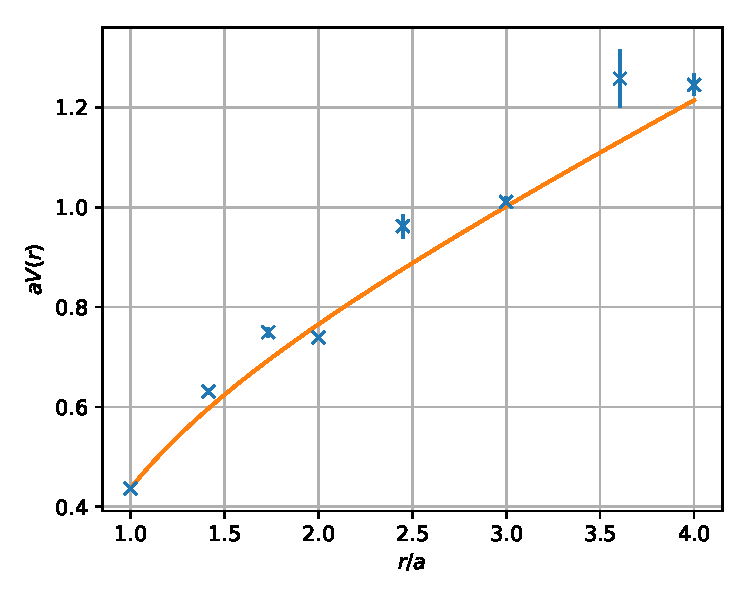
\includegraphics[width=.7\textwidth]{aVfitBeta23.pdf}
    \caption{Das statische Potential in Abhängigkeit vom Abstand von Quark und
    Antiquark: Es ist klar ein linearer Zusammenhang erkennbar.}
    \label{fig:aVfit}
\end{figure}

Die oben beschriebene Messung von $\overline{W(r,t)}$ wurde für
$(r, t) \in \{1, \sqrt{2} \approx 1.4, \sqrt{3} \approx 1.7, 2, \sqrt{6} \approx 2.4,  3, \sqrt{13} \approx 3.6, 4\} \times \{1,2,3,4,5,6,7,8,9\}$
durchgeführt. Für die verschiedenen $r$-Werte wurde nach dem beschriebenen
Verfahren $a V(r)$ bestimmt. Das Resultat ist in Abb. \ref{fig:aVfit} dargestellt.
Die Schlussfolgerung ist klar: Das Potential enthält deutlich einen linearen Term.
Passt man eine Funktion der Form
\[
    a V(r) = -\frac{A}{r} + B + \sigma \cdot r
\]
an die Daten ab, so erhält man
\[
    \sigma = (0.189\pm 0.010) \frac{1}{a}
\]
für die sog. string tension\footnote{Das Potential hat Dimension $L^{-1}$,
dementsprechend ist in der hier gewählten Form $[\sigma] = L^{-1}$.}. Es fällt auf,
dass die Fitkurve nur zwei Fehlerbalken der Datenpunkte direkt schneidet
($\chi^2 = 16.6$). Dies
könnte zweierlei Gründe haben: Auf der einen Seite könnten die Fehler unterschätzt
werden. Diese wurden über den Standardfehler auf das arithmetische Mittel abgeschätzt.
Hier böten andere Methoden (e.\,g. Bootstrap) ggf. bessere Abschätzungen des Fehlers.
Auf der anderen Seite fällt bei genauerer Betrachtung auf, dass die vier Datenpunkte
für ganzzahliges $r/a$ fast perfekt auf einer Linie liegen. Die Datenpunkte für
nichtganzzahlige $r/a$ weichen hiervon ab, da sie von der gewählten Form der
nichtplanaren Loops abhängen. Hier könnte man dadurch Abhilfe schaffen, dass man
verschiedene Formen für die nichtplanaren Wilsonloops vermisst und am Ende über 
die Ergebnisse mittelt. Insgesamt kann aber trotzdem ein linearer Zusammenhang
erkannt werden.

Nun stellt sich natürlich die Frage nach den physikalischen Implikationen dieses
Ergebnisses. Zunächst ist festzustellen, dass die SU(2)-Symmetrie keine alleinige
Wurzel der bekannten Wechselwirkungen darstellt. Insofern kann die gewonnene
Erkenntnis nur in ihrem Analogon zur SU(3)-Symmetrie und der daraus
\enquote{gewonnenen} Quantenchromodymanik verstanden werden. Klar ist: Für die
Parameter $\beta = 2.3$ und $N_\text{t} = 10$ konnte Confinement nachgewiesen
werden. Interpretiert man das untersuchte Gitter als ein tatsächliches
Kristallgitter im Rahmen der statistischen Mechanik (die durchgeführten
Simulationen sind hierzu äquivalent), so kann man das gewonnene Ergebnis als Teil
eines Phasenüberganges bei endlicher Temperatur betrachten. In diesem Fall ist die
Temperatur durch $\theta = \frac{1}{N_\text{t}}$ gegeben und die zwei Phasen
lassen sich als \enquote{Confinement} ($\theta$ klein) und \enquote{Deconfinement}
($\theta$ groß) klassifizieren.

%Nun stellt sich natürlich die Frage nach den physikalischen Implikationen dieses
%Ergebnisses. Die SU(2)-Symmetrie ist nicht alleinige Wurzel einer einzelnen
%Wechselwirkung, vielmehr wird sie im Rahmen der Vereinigung der elektromagetischen
%mit der schwachen Wechselwirkung verwendet, die von SU(2)$\times$U(1) generiert
%wird. Diese Vereinheitlichung ist jedoch erst oberhalb einer bestimmten
%Energieskale resp. unterhalb einer bestimmten Längenskale sinnvoll. Gleichzeitig
%ist zu beachten, dass Confinement aufgrund der laufenden Kopplung nur bei
%kleinen Energien, i.\,e. großen Kopplungen auftritt. (Dies gilt auch für SU(3)
%und die starke Wechselwirkung: Hier spricht man im Gegensatz zu Confinement bei
%kleinen Energien von \emph{asymptotischer Freiheit} bei großen Energien, wo die
%Kopplung schwächer wird und Quarks nur noch leichtinteragierend sind.) Diese beiden
%Erkenntnisse zusammengenommen, ist zu schlussfolgern, dass bei den für die Realität
%relevanten Energieskalen Confinement nicht auftritt.

% !TEX root = mythesis.tex

%==============================================================================
\chapter{Fazit}
\label{sec:fazit}
%==============================================================================

Um den Ansatz für die vorgestellte Demonstration von Confinement im Rahmen der
SU(2)-Eichsymmetrie nachvollziehen zu können, waren zunächst die theoretischen
Hintergründe notwendig. Hierbei wurde als Erstes der Metropolis-Algorithmus
vorgestellt, welcher das fundamentale Werkzeug zur numerischen Approximation
beliebiger Feynman-Pfadintegrale darstellt. Damit wurde als Nächstes exemplarisch
der harmonische Oszillator vorgestellt, hier konnten Grundzustandsenergie und
-wellenfunktion erfolgreich mit Simulationen angenähert werden.

Nun folgte die Betrachtung des von Wilson vorgelegten gitterfeldtheoretischen
Pendants zur Yang-Mills-Wirkung, welches die Dynamik des Eichfelds der
SU(2)-Eichsymmetrie auf einem Gitter beschreibt. Dies ermöglichte dann die
Betrachtung dieser Dynamik mit Hilfe des Metropolisalgorithmus sowie der
Definition der Wilson-Loops als Observable zur Bestimmung des statischen
Potentials eines Quark-Antiquark-Paares.

Die Beschränkung auf SU(2) hatte den Vorteil, dass sich die Eichtransformationen
und die gitterfeldtheoretische Formulierung des Eichfeldes in Form von
Paralleltransporten relativ leicht als unitäre $2 \times 2$-Matrizen mit
Determinante 1 numerisch darstellen ließen. Die Implementierung erfolgte dann
mit C++, es wurden Simulationen auf einem Gitter mit $10^4$ Gitterpunkten
zur Vermessung von Wilson-Loops verschiedener Maße vorgenommen.

Schließlich konnte im Rahmen der Auswertung das statische Potential aus den
gewonnenen Daten extrahiert werden. Der daran vorgenommene Fit zeigte, dass
die ausgeführten Messungen noch verbesserungswürdig sind. Trotzdem konnte
deutlich ebenjener linearer Term im statischen Potential wiedergefunden werden,
den Wilson (wie eingangs erwähnt) ursprünglich vorhergesagt hatte. So konnte
numerisch das Auftreten von Confinement im Rahmen der SU(2)-Eichsymmetrie
nachvollzogen werden.

Leider ist diese Erkenntnis für die physikalische Realität nicht direkt
relevant, da nicht die SU(3)-Eichsymmetrie betrachtet wurde. Die vorgestellten
Konzepte ließen sich aber auch dieses Problem übertragen, hierfür wäre vorallem
eine numerische Repräsentation von Elementen dieser Gruppe notwendig. Alternativ
bietet sich für eine weitergehende Betrachtung die genauere Untersuchung des
Phasenübergangs zwischen Confinement und Deconfinement an.

%Leider ist diese Erkenntnis für die physikalische Realität nur insofern
%bedingt relevant, alsdass die Energieskala, bei der Confinement auftritt weit
%unter der liegt, ab der die elektroschwache Vereinheitlichung ihren
%Gültigkeitsbereich hat, welche von SU(2)$\times$U(1) generiert wird.
%Als nächster Schritt wäre deshalb eine Betrachtung der SU(3)-Eichsymmetrie
%naheliegend, um tatsächlich Confinement für die starke Wechselwirkung zu
%demonstrieren.

% Uncomment the following command to get references per chapter.
% Put it inside the file or change \include to \input if you do not want the references
% on a separate page
% \printbibliography[heading=subbibliography]

%------------------------------------------------------------------------------
% Include the following lines and comment out \printbibliography if
% you use BiBTeX for the bibliography.
% If you use biblatex package the files should be specified in the preamble.
% \KOMAoptions{toc=bibliography}
% {\raggedright
%   \bibliographystyle{../refs/atlasBibStyleWithTitle.bst}
%   % \bibliographystyle{unsrt}
%   \bibliography{./thesis_refs,../refs/standard_refs-bibtex}
% }

%------------------------------------------------------------------------------
\appendix
% \part*{Appendix}
% Add your appendices here - don't forget to also add them to \includeonly above
% !TEX root = mythesis.tex

%------------------------------------------------------------------------------
\chapter{Zusätzliche Graphen}
\label{sec:graphs}
%------------------------------------------------------------------------------

\begin{figure}[htbp]
    \label{fig:beta23a}
    \centering
    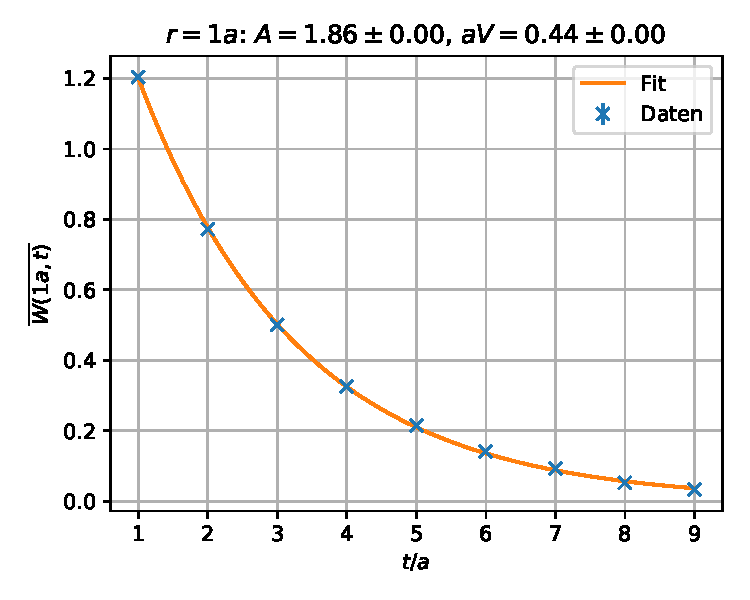
\includegraphics[width=.45\textwidth]{loopResultsBeta23r1}
    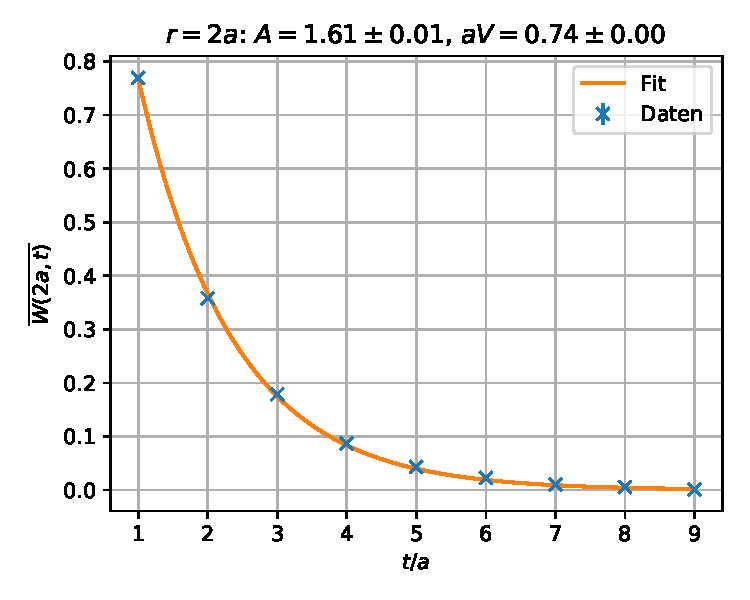
\includegraphics[width=.45\textwidth]{loopResultsBeta23r2}
    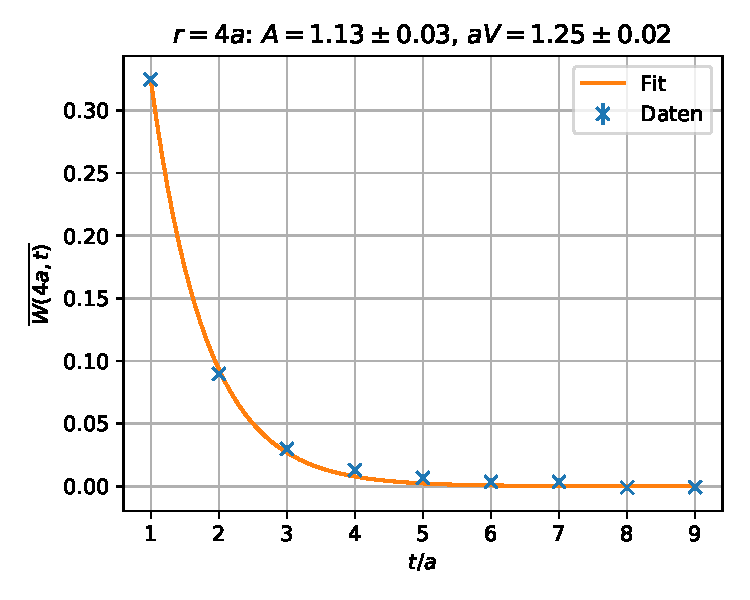
\includegraphics[width=.45\textwidth]{loopResultsBeta23r4}
    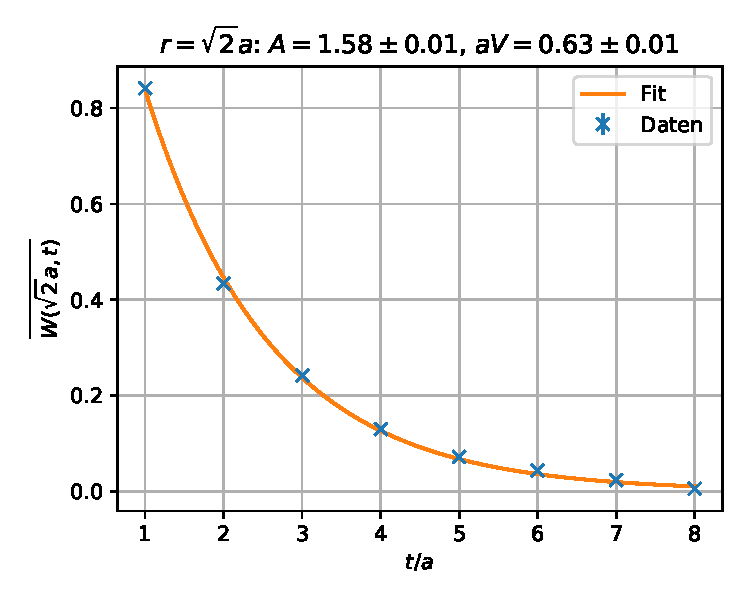
\includegraphics[width=.45\textwidth]{loopResultsBeta23rSqrt2}
    \caption{Messwerte der Wilson-Loops bei $\beta=2.3$ und festegehaltenem
    $r$. Verwendetes Modell: $\overline{W(r,t)} = A \cdot \exp(-aV(r) t/a)$.}
\end{figure}

\begin{figure}[htbp]
    \label{fig:beta23b}
    \centering
    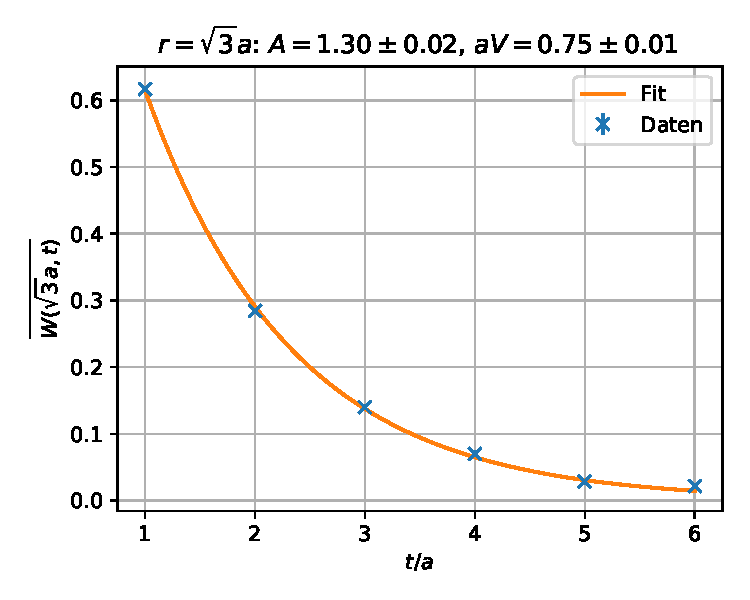
\includegraphics[width=.45\textwidth]{loopResultsBeta23rSqrt3}
    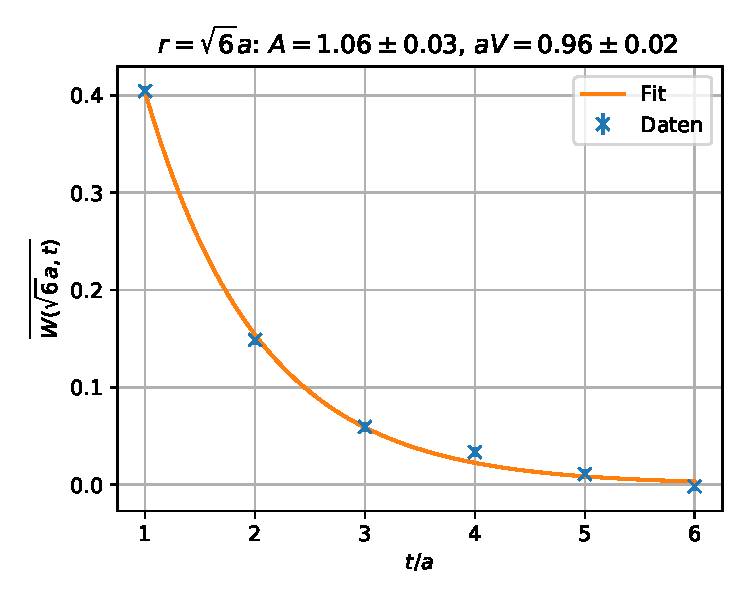
\includegraphics[width=.45\textwidth]{loopResultsBeta23rSqrt6}
    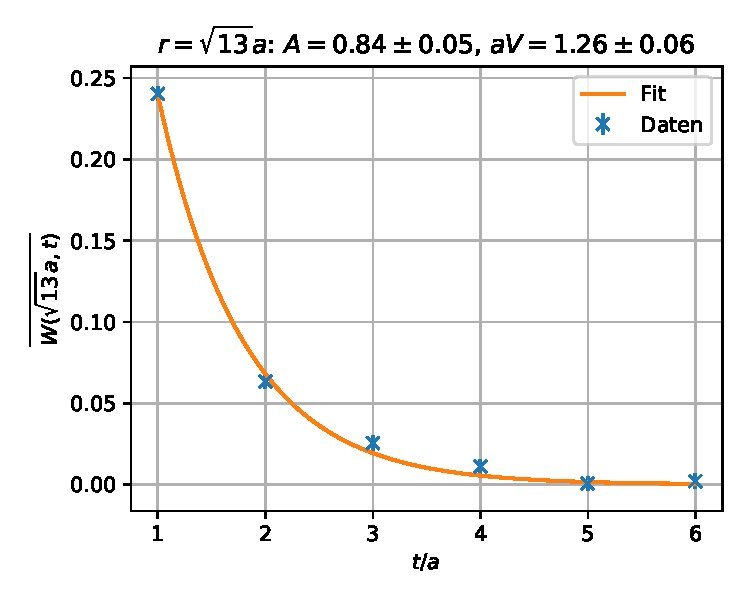
\includegraphics[width=.45\textwidth]{loopResultsBeta23rSqrt13}
    \caption{Messwerte der Wilson-Loops bei $\beta=2.3$ und festegehaltenem
    $r$. Verwendetes Modell: $\overline{W(r,t)} = A \cdot \exp(-aV(r) t/a)$.}
\end{figure}

%------------------------------------------------------------------------------
\chapter{Wertetabellen}
\label{sec:params}
%------------------------------------------------------------------------------

\begin{table}[htbp]
\begin{tabular}{crcl} 
\hline
    $t/a$ &\multicolumn{3}{c}{$\overline{W(a,t)}$} \\ 
\hline
$1$ &	$1.202$ & 	 $\pm$ & 	 $0.002$\\ 
$2$ &	$0.771$ & 	 $\pm$ & 	 $0.003$\\ 
$3$ &	$0.500$ & 	 $\pm$ & 	 $0.003$\\ 
$4$ &	$0.333$ & 	 $\pm$ & 	 $0.004$\\ 
$5$ &	$0.227$ & 	 $\pm$ & 	 $0.005$\\ 
$6$ &	$0.145$ & 	 $\pm$ & 	 $0.005$\\ 
$7$ &	$0.099$ & 	 $\pm$ & 	 $0.005$\\ 
$8$ &	$0.055$ & 	 $\pm$ & 	 $0.005$\\ 
$9$ &	$0.031$ & 	 $\pm$ & 	 $0.005$\\ 
\hline
\end{tabular}
    \hspace{1cm}
\begin{tabular}{crcl} 
\hline
    $t/a$ &\multicolumn{3}{c}{$\overline{W(2a,t)}$} \\ 
\hline
$1$ &	$0.769$ & 	 $\pm$ & 	 $0.003$\\ 
$2$ &	$0.366$ & 	 $\pm$ & 	 $0.003$\\ 
$3$ &	$0.182$ & 	 $\pm$ & 	 $0.003$\\ 
$4$ &	$0.086$ & 	 $\pm$ & 	 $0.003$\\ 
$5$ &	$0.041$ & 	 $\pm$ & 	 $0.003$\\ 
$6$ &	$0.021$ & 	 $\pm$ & 	 $0.005$\\ 
$7$ &	$0.004$ & 	 $\pm$ & 	 $0.005$\\ 
$8$ &	$0.008$ & 	 $\pm$ & 	 $0.005$\\ 
$9$ &	$0.004$ & 	 $\pm$ & 	 $0.005$\\ 
\hline
\end{tabular}
    \hspace{1cm}
\begin{tabular}{crcl} 
\hline
    $t/a$ &\multicolumn{3}{c}{$\overline{W(3a,t)}$} \\ 
\hline
$1$ &	$0.498$ & 	 $\pm$ & 	 $0.003$\\
$2$ &	$0.176$ & 	 $\pm$ & 	 $0.003$\\
$3$ &	$0.068$ & 	 $\pm$ & 	 $0.003$\\
$4$ &	$0.025$ & 	 $\pm$ & 	 $0.005$\\
$5$ &	$0.019$ & 	 $\pm$ & 	 $0.005$\\
$6$ &	$0.004$ & 	 $\pm$ & 	 $0.005$\\
$7$ &	$0.013$ & 	 $\pm$ & 	 $0.005$\\
$8$ &	$0.007$ & 	 $\pm$ & 	 $0.005$\\
$9$ &	$-0.004$ & 	 $\pm$ & 	 $0.005$\\
\hline
\end{tabular}
    \caption{Wertetabellen für die Messungen der Wilson-Loops bei $\beta = 2.3$.
    Nach 1000 Sweeps zur Equilibrierung wurden die Messungen jeweils mit 5 sweeps
    Abstand genommen, um Korrelation zu reduzieren.}
    \label{tab:wilsonBeta23a}
\end{table}

\begin{table}[htbp]
\begin{tabular}{crcl} 
\hline
    $t/a$ &\multicolumn{3}{c}{$\overline{W(4a,t)}$} \\ 
\hline
$1$ &	$0.327$ & 	 $\pm$ & 	 $0.003$\\
$2$ &	$0.090$ & 	 $\pm$ & 	 $0.003$\\
$3$ &	$0.027$ & 	 $\pm$ & 	 $0.003$\\
$4$ &	$0.007$ & 	 $\pm$ & 	 $0.005$\\
$5$ &	$0.002$ & 	 $\pm$ & 	 $0.005$\\
$6$ &	$0.009$ & 	 $\pm$ & 	 $0.005$\\
$7$ &	$0.011$ & 	 $\pm$ & 	 $0.005$\\
$8$ &	$-0.002$ & 	 $\pm$ & 	 $0.005$\\
$9$ &	$-0.009$ & 	 $\pm$ & 	 $0.005$\\
\hline
\end{tabular}
    \hspace{1cm}
\begin{tabular}{crcl} 
\hline
    $t/a$ &\multicolumn{3}{c}{$\overline{W(\sqrt{2}a,t)}$} \\ 
\hline
$1$ &	$0.841$ & 	 $\pm$ & 	 $0.004$\\
$2$ &	$0.434$ & 	 $\pm$ & 	 $0.004$\\
$3$ &	$0.241$ & 	 $\pm$ & 	 $0.004$\\
$4$ &	$0.130$ & 	 $\pm$ & 	 $0.004$\\
$5$ &	$0.071$ & 	 $\pm$ & 	 $0.004$\\
$6$ &	$0.043$ & 	 $\pm$ & 	 $0.004$\\
$7$ &	$0.023$ & 	 $\pm$ & 	 $0.004$\\
$8$ &	$0.005$ & 	 $\pm$ & 	 $0.004$\\
\hline
\end{tabular}
    \hspace{1cm}
\begin{tabular}{crcl} 
\hline
    $t/a$ &\multicolumn{3}{c}{$\overline{W(\sqrt{3}a,t)}$} \\ 
\hline
$1$ &	$0.617$ & 	 $\pm$ & 	 $0.004$\\
$2$ &	$0.285$ & 	 $\pm$ & 	 $0.004$\\
$3$ &	$0.140$ & 	 $\pm$ & 	 $0.004$\\
$4$ &	$0.070$ & 	 $\pm$ & 	 $0.004$\\
$5$ &	$0.028$ & 	 $\pm$ & 	 $0.004$\\
$6$ &	$0.022$ & 	 $\pm$ & 	 $0.004$\\
\hline
\end{tabular}
    \caption{Wertetabellen für die Messungen der Wilson-Loops bei $\beta = 2.3$.
    Nach 1000 Sweeps zur Equilibrierung wurden die Messungen jeweils mit 5 sweeps
    Abstand genommen, um Korrelation zu reduzieren.}
    \label{tab:wilsonBeta23b}
\end{table}

\begin{table}[htbp]
\begin{tabular}{crcl} 
\hline
    $t/a$ &\multicolumn{3}{c}{$\overline{W(\sqrt{6}a,t)}$} \\ 
\hline
$1$ &	$0.404$ & 	 $\pm$ & 	 $0.004$\\
$2$ &	$0.149$ & 	 $\pm$ & 	 $0.005$\\
$3$ &	$0.060$ & 	 $\pm$ & 	 $0.005$\\
$4$ &	$0.033$ & 	 $\pm$ & 	 $0.005$\\
$5$ &	$0.011$ & 	 $\pm$ & 	 $0.005$\\
$6$ &	$-0.002$ & 	 $\pm$ & 	 $0.005$\\
\hline
\end{tabular}
    \hspace{1cm}
\begin{tabular}{crcl} 
\hline
    $t/a$ &\multicolumn{3}{c}{$\overline{W(\sqrt{13}a,t)}$} \\ 
\hline
$1$ &	$0.240$ & 	 $\pm$ & 	 $0.004$\\ 
$2$ &	$0.063$ & 	 $\pm$ & 	 $0.004$\\ 
$3$ &	$0.025$ & 	 $\pm$ & 	 $0.004$\\ 
$4$ &	$0.011$ & 	 $\pm$ & 	 $0.004$\\ 
$5$ &	$0.001$ & 	 $\pm$ & 	 $0.004$\\ 
$6$ &	$0.002$ & 	 $\pm$ & 	 $0.004$\\ 
\hline
\end{tabular}
    \caption{Wertetabellen für die Messungen der Wilson-Loops bei $\beta = 2.3$.
    Nach 1000 Sweeps zur Equilibrierung wurden die Messungen jeweils mit 5 sweeps
    Abstand genommen, um Korrelation zu reduzieren.}
    \label{tab:wilsonBeta23c}
\end{table}

% \printbibliography[heading=subbibliography]

%------------------------------------------------------------------------------
% Use biblatex for the bibliography
% Add bibliography to Table of Contents
% Comment out this command if your references are printed for each chapter.
\printbibliography[heading=bibintoc]

%------------------------------------------------------------------------------
% Declare lists of figures and tables and acknowledgements as backmatter
% Chapter/section numbers are turned off
\backmatter

%\listoffigures

%------------------------------------------------------------------------------
% Print the glossary and list of acronyms
% \printglossaries

%------------------------------------------------------------------------------
% You could instead add your acknowledgements here - don't forget to
% also add them to \includeonly above
% %------------------------------------------------------------------------------
\chapter*{Acknowledgements}
\label{sec:ack}
%------------------------------------------------------------------------------

I would like to thank ...

You should probably use \texttt{\textbackslash chapter*} for
acknowledgements at the beginning of a thesis and
\texttt{\textbackslash chapter} for the end.

%%% Local Variables: 
%%% mode: latex
%%% TeX-master: "../mythesis"
%%% End: 


%------------------------------------------------------------------------------
% CV needed when you submit your PhD thesis
% \definecolor{lightgray}{gray}{0.8}
\newcolumntype{L}{>{\raggedleft}p{0.15\textwidth}}
\newcolumntype{R}{p{0.8\textwidth}}
\newcommand\VRule{\color{lightgray}\vrule width 0.5pt}

\thispagestyle{empty}
\section*{Curriculum Vitae}

\subsection*{Personal Details}

\begin{tabular}{L!{\VRule}R}
Name & Johann Schmidt \\
Date of Birth &  \\
Email & abc@physik.uni-def.de \\
Family status & Single
\end{tabular}

\subsection*{Education}

\begin{tabular}{L!{\VRule}R}
1997--2003 & Abitur, ABC Secondary School, Hamburg, Germany\\
2004--2007 & BSc in Physics, Rheinische Friedrich-Wilhelms-Universität, Bonn, Germany.\\
2006 & CERN Summer Student, Geneva, Switzerland. \\
2007--2009 &  MSc in Physics Rheinische Friedrich-Wilhelms-Universität, Bonn, Germany. \\
2009--2012 &  PhD in Physics, Rheinische Friedrich-Wilhelms-Universität, Bonn, Germany. \\
2012 & Advanced Data Analysis School, Frankfurt, Germany.
\end{tabular}

\subsection*{Professional Experience}

\begin{tabular}{L!{\VRule}R}
2004 & Summer Student at CERN, Geneva, Switzerland. \\
2007--2012 & Doctoral work at the University of Bonn, Germany. \\
2008--2009 & Fieldwork at CERN, Geneva, Switzerland.\\
2011 & Talk at the Advanced Physics Conference, Timbucto
\end{tabular}

\subsection*{Languages}
\begin{tabular}{L!{\VRule}R}
German & Mother tongue \\
English & Fluent \\
Russian & Basic
\end{tabular}


\end{document}
